\documentclass[leqno, openany]{memoir}
\setulmarginsandblock{3.5cm}{3.5cm}{*}
\setlrmarginsandblock{3cm}{3.5cm}{*}
\checkandfixthelayout

\usepackage{amsmath}
\usepackage{amssymb}
\usepackage{amsthm}
%\usepackage{MnSymbol}
\usepackage{bm}
\usepackage{accents}
\usepackage{mathtools}
\usepackage{tikz}
\usetikzlibrary{calc}
\usetikzlibrary{automata,positioning}
\usepackage{tikz-cd}
\usepackage{forest}
\usepackage{braket} 
\usepackage{listings}
\usepackage{mdframed}
\usepackage{verbatim}
\usepackage{physics}
\usepackage{stmaryrd}
\usepackage{mathrsfs} 
\usepackage{ulem} 
%\usepackage{/home/patrickl/homework/macaulay2}

%font
\usepackage[sc]{mathpazo}
\usepackage{eulervm}
\usepackage[scaled=0.86]{berasans}
\usepackage{inconsolata}
\usepackage{microtype}

%CS packages
\usepackage{algorithmicx}
\usepackage{algpseudocode}
\usepackage{algorithm}

% typeset and bib
\usepackage[english]{babel} 
\usepackage[utf8]{inputenc} 
\usepackage[T1]{fontenc}
\usepackage[backend=biber, style=alphabetic]{biblatex}
\usepackage[bookmarks, colorlinks, breaklinks]{hyperref} 
\hypersetup{linkcolor=black,citecolor=black,filecolor=black,urlcolor=blue}

% other formatting packages
\usepackage{float}
\usepackage{booktabs}
\usepackage[shortlabels]{enumitem}
\usepackage{csquotes}
\usepackage{titlesec}
\usepackage{titling}
% \usepackage{fancyhdr}
% \usepackage{lastpage}
\usepackage{parskip}

\usepackage{lipsum}

% delimiters
\DeclarePairedDelimiter{\gen}{\langle}{\rangle}
\DeclarePairedDelimiter{\floor}{\lfloor}{\rfloor}
\DeclarePairedDelimiter{\ceil}{\lceil}{\rceil}


\newtheorem{thm}{Theorem}[section]
\newtheorem{cor}[thm]{Corollary}
\newtheorem{prop}[thm]{Proposition}
\newtheorem{lem}[thm]{Lemma}
\newtheorem{conj}[thm]{Conjecture}
\newtheorem{quest}[thm]{Question}

\theoremstyle{definition}
\newtheorem{defn}[thm]{Definition}
\newtheorem{defns}[thm]{Definitions}
\newtheorem{con}[thm]{Construction}
\newtheorem{exm}[thm]{Example}
\newtheorem{exms}[thm]{Examples}
\newtheorem{notn}[thm]{Notation}
\newtheorem{notns}[thm]{Notations}
\newtheorem{addm}[thm]{Addendum}
\newtheorem{exer}[thm]{Exercise}

\theoremstyle{remark}
\newtheorem{rmk}[thm]{Remark}
\newtheorem{rmks}[thm]{Remarks}
\newtheorem{warn}[thm]{Warning}
\newtheorem{sch}[thm]{Scholium}


% unnumbered theorems
\theoremstyle{plain}
\newtheorem*{thm*}{Theorem}
\newtheorem*{prop*}{Proposition}
\newtheorem*{lem*}{Lemma}
\newtheorem*{cor*}{Corollary}
\newtheorem*{conj*}{Conjecture}

% unnumbered definitions
\theoremstyle{definition}
\newtheorem*{defn*}{Definition}
\newtheorem*{exer*}{Exercise}
\newtheorem*{defns*}{Definitions}
\newtheorem*{con*}{Construction}
\newtheorem*{exm*}{Example}
\newtheorem*{exms*}{Examples}
\newtheorem*{notn*}{Notation}
\newtheorem*{notns*}{Notations}
\newtheorem*{addm*}{Addendum}


\theoremstyle{remark}
\newtheorem*{rmk*}{Remark}

% shortcuts
\newcommand{\Ima}{\mathrm{Im}}
\newcommand{\Gr}{\mathrm{Gr}}
\newcommand{\A}{\mathbb{A}}
\newcommand{\F}{\mathbb{F}}
\newcommand{\G}{\mathbb{G}}
\newcommand{\N}{\mathbb{N}}
\newcommand{\R}{\mathbb{R}}
\newcommand{\C}{\mathbb{C}}
\newcommand{\Z}{\mathbb{Z}}
\newcommand{\Q}{\mathbb{Q}}
\renewcommand{\k}{\Bbbk}
\renewcommand{\P}{\mathbb{P}}
\newcommand{\M}{\overline{M}}
\newcommand{\g}{\mathfrak{g}}
\newcommand{\h}{\mathfrak{h}}
\newcommand{\n}{\mathfrak{n}}
\renewcommand{\b}{\mathfrak{b}}
\newcommand{\ep}{\varepsilon}
\newcommand*{\dt}[1]{%
   \accentset{\mbox{\Huge\bfseries .}}{#1}}
\renewcommand{\abstractname}{Official Description}
\newcommand{\mc}[1]{\mathcal{#1}}
\newcommand{\T}{\mathbb{T}}
\newcommand{\mf}[1]{\mathfrak{#1}}
\newcommand{\mr}[1]{\mathrm{#1}}
\newcommand{\ms}[1]{\mathsf{#1}}
\newcommand{\on}[1]{\operatorname{#1}}
\newcommand{\ol}[1]{\overline{#1}}
\newcommand{\ul}[1]{\underline{#1}}
\newcommand{\wt}[1]{\widetilde{#1}}
\newcommand{\wh}[1]{\widehat{#1}}
\renewcommand{\div}{\operatorname{div}}
\newcommand{\bir}{\sim_{\mr{bir}}}
\newcommand{\stacks}[1]{\href{https://stacks.math.columbia.edu/tag/#1}{#1}}

\DeclareMathOperator{\Der}{Der}
\DeclareMathOperator{\Def}{Def}
\DeclareMathOperator{\Bl}{Bl}
\DeclareMathOperator{\NE}{NE}
\DeclareMathOperator{\Tor}{Tor}
\DeclareMathOperator{\Hom}{Hom}
\DeclareMathOperator{\Ext}{Ext}
\DeclareMathOperator{\End}{End}
\DeclareMathOperator{\ad}{ad}
\DeclareMathOperator{\Aut}{Aut}
\DeclareMathOperator{\Rad}{Rad}
\DeclareMathOperator{\Pic}{Pic}
\DeclareMathOperator{\Alb}{Alb}
\DeclareMathOperator{\supp}{supp}
\DeclareMathOperator{\Supp}{Supp}
\DeclareMathOperator{\sgn}{sgn}
\DeclareMathOperator{\spec}{Spec}
\DeclareMathOperator{\Spec}{Spec}
\DeclareMathOperator{\proj}{Proj}
\DeclareMathOperator{\Proj}{Proj}
\DeclareMathOperator{\ord}{ord}
\DeclareMathOperator{\Div}{Div}
\DeclareMathOperator{\depth}{depth}
\DeclareMathOperator{\coker}{coker}
\DeclareMathOperator{\rk}{rk}
\DeclareMathOperator{\Sym}{Sym}

% Section formatting
\titleformat{\section}
    {\Large\sffamily\scshape\bfseries}{\thesection}{1em}{}
\titleformat{\subsection}[runin]
    {\large\sffamily\bfseries}{\thesubsection}{1em}{}
\titleformat{\subsubsection}[runin]{\normalfont\itshape}{\thesubsubsection}{1em}{}

\title{COURSE TITLE}
\author{Lectures by INSTRUCTOR, Notes by NOTETAKER}
\date{SEMESTER}

\newcommand*{\titleSW}
    {\begingroup% Story of Writing
    \raggedleft
    \vspace*{\baselineskip}
    {\Huge\itshape Hyperbolicity Graduate Student Seminar \\ Spring 2022}\\[\baselineskip]
    {\large\itshape Notes by Patrick Lei}\\[0.2\textheight]
    {\Large Lectures by Various}\par
    \vfill
    {\Large \sffamily Columbia University}
    \vspace*{\baselineskip}
\endgroup}
\pagestyle{simple}

\chapterstyle{ell}


%\renewcommand{\cftchapterpagefont}{}
\renewcommand\cftchapterfont{\sffamily}
\renewcommand\cftsectionfont{\scshape}
\renewcommand*{\cftchapterleader}{}
\renewcommand*{\cftsectionleader}{}
\renewcommand*{\cftsubsectionleader}{}
\renewcommand*{\cftchapterformatpnum}[1]{~\textbullet~#1}
\renewcommand*{\cftsectionformatpnum}[1]{~\textbullet~#1}
\renewcommand*{\cftsubsectionformatpnum}[1]{~\textbullet~#1}
\renewcommand{\cftchapterafterpnum}{\cftparfillskip}
\renewcommand{\cftsectionafterpnum}{\cftparfillskip}
\renewcommand{\cftsubsectionafterpnum}{\cftparfillskip}
\setrmarg{3.55em plus 1fil}
\setsecnumdepth{subsection}
\maxsecnumdepth{subsection}
\settocdepth{subsection}

\begin{document}
    
\begin{titlingpage}
\titleSW
\end{titlingpage}

\thispagestyle{empty}
\section*{Disclaimer}%
\label{sec:disclaimer}

These notes were taken during the seminar using the \texttt{vimtex} package of the editor \texttt{neovim}. 
Any errors are mine and not the speakers'. 
In addition, my notes are picture-free (but will include commutative diagrams) and are a mix of my mathematical style and that of the lecturers.
If you find any errors, please contact me at \texttt{plei@math.columbia.edu}.

\section*{Acknowledgements}
I would like to thank Amal Mattoo for pointing out mistakes and corrections in these notes.

\vspace*{1cm}

\noindent\textbf{Seminar Website:}  \url{https://www.math.columbia.edu/~dejong/seminar/seminar-hyperbolicity.html}
\newpage

\tableofcontents

\chapter{Akash (Feb 04): Introduction}%

Throughout this lecture, we will be working in characteristic 0. In dimension $1$, let $X$ be a smooth projective curve of genus $g \geq 2$. Consider the following four properties: 
\begin{enumerate}[(1)]
    \item Then $K_X$ is ample, so 
    \[ h^0 (X, m K_X) = m (2g-2) + 1-g = O(m) \]
    by Riemann-Roch. 
    \item If we consider $X$ as a curve over $\C$, then the corresponding Riemann surface has a hyperbolic metric. 
    \item By uniformization, the universal cover of $X$ is the disc $\mathbb{D}$. By basic algebraic topology, any holomorphic map $f \colon \C \to X$ is constant. 
    \item Now, if $X$ is a curve over a number field $F$, then by Faltings, $X(F)$ is finite. All of these properties fail if $g \leq 1$, and so we would like to generalize them to higher dimensions.
\end{enumerate}

\section{Kobayashi and Brody hyperbolicity}
Consider the unit disc $D \subseteq \C$. Then there is a metric
\[ \frac{\dd{z} \wedge \dd{\ol{z}}}{(1-\abs{z}^2)^2}. \]
This tells us that for $u_z \in T_z$, we have
\[ \norm{v}_{\mr{hyp}} = \frac{\norm{u}_{\mr{clas}}}{(1-\abs{z}^2)^2}, \]
which gives us a metric (in the sense of a metric space) on $D$. If $X$ is a curve of genus $g \geq 2$, then the metric is preserved by the action of the fundamental group of $X$, so the hyperbolic metric descends to $X$.

\begin{prop}
    Let $f \colon D \to D$. Then $f$ non-increases the distance for the hyperbolic metric.
\end{prop}

\begin{proof}
    By the Schwarz lemma, we have
    \[ \frac{\abs{f'(z)}}{1-\abs{f(z)}^2} \leq \frac{1}{1-\abs{z}^2}, \]
    and this gives the desired result.
\end{proof}

Now let $X$ be a complex manifold. Then for points $x, y \in X$, we will connect them by a series of holomorphic discs $f_i \colon D \to X$ with $p_i, q_i \in D$ such that $f_1(p_1) = x, f_m(q_m) = y$, and $f_i(q_i) = f_{i+1}(p_{i+1})$. Then considering all such paths, we define
\[ d_X(x, y) = \inf \sum_{i=1}^m d_{\mr{hyp}}(p_i, q_i). \]
This might not be a metric because for $X = \C$, $d_X(x,y) = 0$ for any $x,y$. Here, we simply consider $f_n(z) = n(y-x) z + x$. This sends $0$ to $x$ and $1/n$ to $y$, so by approximating the hyperbolic metric with the Euclidean metric, we see that $d_X(x,y) = 0$. On the other hand, if $X$ is a compact Riemann surface of genus $g \geq 2$, then $d_X$ is a metric.

\begin{defn}
    Let $X$ be a complex manifold. Then $X$ is \textit{Kobayashi hyperbolic} if $d_X$ is a metric.
\end{defn}

Some non-examples are $\P^n$, abelian varieties, rationally connected varieties, and K3 surfaces. More generally, if there is a nontrivial holomorphic $f \colon \C \to X$, then $X$ is not hyperbolic.

\begin{thm}[Brody]
    The converse holds when $X$ is compact.
\end{thm}

\begin{defn}
    Let $X$ be a complex manifold. Then $X$ is \textit{Brody hyperbolic} if any holomorphic map $f \colon \C \to X$ is constant.
\end{defn}

Therefore, the theorem can be rephrased as saying that Brody hyperbolicity is equivalent to Kobayashi hyperbolicity for compact manifolds.

Let $f \colon D \to X$. Then $\dd{f(z)} \colon T_z D \to T_{f(z)} X$, and so we have
\[ \abs{\dd{f}(z)} = \sup \frac{\abs{\dd{f(z)} v}_{\mr{her}}}{\abs{v}_{\mr{hyp}}}. \]
Then we define
\[ C(f) = \sup_{z \in D} \abs{\dd{f(z)}} \]
and taking the supremum of all maps to $X$, we have
\[ C(X) = \sup_{f \colon D \to X} C(f). \]

Note that if $C(X)$ is finite, then $X$ is Kobayashi hyperbolic. If $X$ is compact, then the converse also holds.

\begin{proof}[Proof of theorem]
    We want to show that if $X$ is not Kobayashi hyperbolic, then there is a holomorphic map $f \colon \C \to X$. We know that there exists $f_n \colon D \to X$ such that $C(f_n) \to \infty$. In particular, $\abs{\dd{f_n(z)}} \to \infty$. Reparameterizing, there exist $f_n \colon D_{r_n} \to X$ such that $\abs{\dd{f(0)}} = 1$ and $r_n \to \infty$. We would like to now construct $f \colon \C \to X$.

    First, for any compact subset $K \subseteq \C$, there exists a subsequence $f_n$ that converges on $K$. We have a subsequence that converges uniformly on $D_1$, to some $f_1$. Taking another subsequence, we obtain $f_2$ on $D_2$. Continuing, we obtain $f \colon \C \to X$.
\end{proof}

\begin{exm}
    If $X \subseteq A$ is contained in an abelian variety, then a theorem of Bloch says that $X$ is hyperbolic if and only if it does not contain the translate of some abelian subvariety of positive dimension.
\end{exm}

\begin{exm}
    Quotients of bounded domains (for example moduli of abelian varieties) are hyperbolic.
\end{exm}

\begin{exm}
    If $X \to Y$ is a smooth projective map to a hyperbolic $Y$ with hyperbolic fibers, then $X$ is hyperbolic.
\end{exm}

\begin{exm}
    If $f \colon X \to Y$ is finite \'etale, then $X$ is hyperbolic if and only if $Y$ is hyperbolic.
\end{exm}

\begin{exm}
    Varieties with ample cotangent bundle are hyperbolic.
\end{exm}

\section{Algebraic hyperbolicity}
\begin{defn}
    Let $X$ be a compact complex manifold with Hermitian metric $h$. Then $X$ is \textit{algebraically hyperbolic} if there exists $\ep > 0$ such that for all $f \colon C \to X$ with $C$ a smooth projective curve, we have
    \[ 2 g(c) - 2 \geq \ep \int_C f^* \omega_h. \]
\end{defn}

For example, if $X$ is smooth and projective with $A$ ample, then $2g(C) - 2 \geq \ep \deg f^* A$. In particular, if $X$ is algebraically hyperbolic, it cannot contain any rational curves or elliptic curves.

\begin{thm}
    Let $X$ be a compact complex manifold. If $X$ is Kobayashi hyperbolic, then it is algebraically hyperbolic.
\end{thm}

\begin{proof}
    Let $f \colon C \to X$. By Gauss-Bonnet, we have
    \[ 2 g(C) - 2 = - \int_C \Theta_{h_C} = \frac{2}{\pi} \int_C \omega_{h_C} \geq \frac{2}{\pi c^2} f^* \omega_h, \]
    where the inequality follows from Kobayashi hyperbolicity.
\end{proof}

\begin{prop}
    Let $X$ be a smooth projective variety over $\C$. If $X$ is algebraically hyperbolic, then any $A \to X$ from an abelian variety $A$ is constant.
\end{prop}

\begin{proof}
    Consider $C \subset A \xrightarrow{m_A} A \xrightarrow{f} X$. Then if we pull back an ample $L$, we can increase the degree of the pullback of $L$ arbitrarily.
\end{proof}

Note that if $\dim X = 2$, then $X$ must be a surface of general type by the classification of surfaces. It is unknown whether or hyperbolicity is equivalent to having every subvariety be of general type.

\section{Rational points}
Let $X$ be a variety over $\ol{\Q}$.
\begin{defn}
    $X$ is \textit{Mordellic} if $X(K)$ is finite for all number fields $K \subseteq \ol{\Q}$.
\end{defn}

If $X$ is smooth and projective, we can consider $X_{\C}$. If $X$ is Mordellic, then $X_{\C}$ should be hyperbolic. Also note that hyperbolicity and Mordellness are not birational invariants (if you blow up a point, you get many rational points and rational curves).

\begin{conj}[Weak Lang]
    A variety $X$ over a number field $K$ is of general type if and only if $X(K')$ is not Zariski dense for all finite extensions $K'/K$.
\end{conj}

\begin{thm}[Caporaso-Harris-Mazur]
    Weak Lang implies a uniform bound on the number of rational points.
\end{thm}

\chapter{Akash (Feb 11): Analytic preliminaries}%

\section{Some conjectures}

Before we start doing analysis, we would like to state some conjectures relating different notions of hyperbolicity. As usual, we will assume that $X$ is smooth and projective over $\C$.

\begin{defn}
    A smooth projective variety $X$ is \textit{groupless} if there is no nonconstant morphism $A \to X$ from an abelian variety $A$.
\end{defn}

We know that Brody and Kobayashi hyperbolicity are equivalent and that Kobayashi hyperbolicity implies algebraic hyperbolicity, which in turn implies grouplessness. Now remember that curves of genus $\geq 2$ are of general type and recall that general type means that $K_X$ is big. The condition that we want is in fact that every subvariety of $X$ is of general type.

\begin{conj}
    The conditions of Brody hyperbolicity, Kobayashi hyperbolicity, algebraic hyperbolicity, Mordellicity, grouplessness, and $X$ being of general type with all subvarieties of general type are equivalent.
\end{conj}

This conjecture is known in dimension $1$. Also, in general, we know that every subvariety of $X$ being of general type and $X$ being Mordellic imply that $X$ is groupless. In dimension $2$, we know that grouplessness, Kobayashi hyperbolicity, and every subvariety being of general type are equivalent (the equivalence of grouplessness and the general type condition is due to the classification of surfaces). Also, if $X$ has ample cotangent bundle, then all of the conditions are satisfied by $X$.

Now note that all of these properties are not birational invariants. If we blow up a point, we obtain a copy of projective space, which has lots of rational curves. To fix this, we will pseudofy the definitions. For example, we will generalize the Mordellic condition to $X \setminus \Delta$ having finitely many rational points for some proper closed subset $\Delta$.

\begin{defn}
    $X$ is \textit{Brody hyperbolic modulo $\Delta$} if for any nonconstant $f \colon \C \to X$, $f(\C) \subseteq \Delta$.
\end{defn}

\begin{defn}
    $X$ is \textit{Kobayashi hyperbolic modulo $\Delta$} if $d_X(x, y) > 0$ for $x \neq y \in X \setminus \Delta$.
\end{defn}

\begin{defn}
    $X$ is \textit{Algebraically hyperbolic modulo $\Delta$} if there exists there exists $\alpha_{X, \Delta, L}$ such that for all $f \colon C \to X$, then $\deg f^* L \leq \alpha_{X, \Delta, L} g(C)$ if $f(C) \not\subseteq \Delta$.
\end{defn}

\begin{defn}
    $X$ is \textit{Mordellic modulo $\Delta$} if $(X \setminus \Delta)(k)$ is finite for any number field $k$.
\end{defn}

\begin{defn}
    $X$ is \textit{Groupless modulo $\Delta$} if any nonconstant $A \dashrightarrow X$ lands inside $\Delta$.
\end{defn}

If there exists a closed $\Delta \subsetneq X$ such that $X$ is hyperbolic modulo $\Delta$, then we say that $X$ is \textit{pseudo-hyperbolic}.

\begin{conj}
    The conditions pseudo-Brody, pseudo-Kobayashi, pseudo-algebraically hyperbolic, pseudo-groupless, pseudo-Mordellic, and general type are equivalent.
\end{conj}

We know that pseudo-Kobayashi implies pseudo-Brody and that pseudo-algebraically hyperbolic implies pseudo-groupless. Also, pseudo-Mordellic implies pseudo-groupless.

In dimension $2$, we know that if $X$ is general type and $c_1^2 > c_2$, then there exist finitely many rational and elliptic curves on $X$ by a result of Bogomolov. Also, by a result of Mcquillen, $X$ is pseudo-Brody.

Now let $\mr{Exc}(X) = \bigcap_{X \text{ hyp mod }\Delta}$ be the exceptional locus. The strongest version of the conjecture is that all exceptional loci agree under the different notions of hyperbolicity. This strongest version is known for subvarieties of abelian varieties. If $X \subseteq A$, then let $\mr{sp}(X)$ be the union of all translates of abelian subvarieties $A' \subseteq A$ that are contained in $X$. Then if we set this to be the exceptional locus, we have this strongest version for $X$ of general type.

\section{Ahlfors-Schwarz lemma}

Let $X$ be a complex manifold and $L$ be a line bundle on $X$ with a metric. Consider $\norm{S}^2 = \frac{\abs{S}_{\mr{euc}}}{f(z)}$. We also have an associated $(1,1)$-form $\omega_h = - \Im h$. We also have a Chern form 
\[ \Theta_h(L) = \frac{i}{2 \pi} \partial \ol{\partial} \log \norm{-}_h, \]
which represents $c_1(L)$. Note that $L$ is ample if $\Theta_L(L) \geq \ep \omega_h$ for some $\ep > 0$ and some metric on $L$.

\begin{exm}
    Let $X = \Delta$ be the disk and $L = T_X$. Then
    \[ h_{\mr{hyp}} = \frac{\dd{z} \otimes \dd{z^2}}{(1-\abs{z}^2)^2}, \]
    and thus
    \[ \omega_{\mr{hyp}} = \frac{i \dd{z} \wedge \dd{\ol{z}}}{(1-\abs{z}^2)^2}. \]
    In this case, we have $\Theta_{\mr{hyp}} = \frac{-1}{\pi} \omega_{\mr{hyp}}$.
\end{exm}

\begin{lem}[Ahlfors-Schwarz]
    Now let $X = D_a$. Then suppose $h = h(z) \dd{z} \otimes \dd{\ol{z}}$ is a Hermitian metric on $D_a$ such that $i \partial \ol{\partial} \log h \geq \ep \omega_h$ for some $\ep > 0$. Then $h \leq \frac{1}{\ep} h_{\mr{hyp}}$.
\end{lem}

\begin{proof}
    Define 
    \[ u(z) = h(z) \frac{( \abs{a}^2 - \abs{z}^2 )^2}{a}. \] 
    We can reparameterize to assume that $u(z)$ is defined on a closed unit disc. Thus, write $u(z) = h(z) (1-\abs{z}^2)$. We know that $u(z) = 0$ on $\partial D$, so it has a maximum in $D_1$ at $z_0 \in D_1$. But now at $z_0, \log u(z)$ has a maximum. Therefore 
    \[\partial \ol{\partial} \log u(z_0) \leq 0. \]

    Therefore, $\partial \ol{\partial} \log h(z_0) - \partial \ol{\partial} \log h_{\mr{hyp}}(z_0) \leq 0$. In particular, we have
    \[ \ep \omega_h(z_0) - \frac{1}{\pi} \omega_{\mr{hyp}}(z_0) \leq 0. \]
    This implies that $(\ep u(z_0) - 1) \omega_{\mr{hyp}}(z_0) \leq 0$. Therefore $u(z_0) \leq \frac{1}{\ep}$.
\end{proof}

We will now discuss how this is used to study hyperbolicity. In particular, we will show that if $X$ has ample cotangent bundle, then $X$ is Brody hyperbolic. Consider $f \colon \C \to X$. There is a lift to $\P T_X = \Proj \on{Sym} \Omega^1_X \eqqcolon P$. On $P$, we know that $L \coloneqq \mc{O}_P(1)$ is ample and that $\pi_* \mc{O}_P(m) = \on{Sym}^m \Omega^1_X$. Also, we know that $H^0(P, \mc{O}_P(m)) = H^0(X, \on{Sym}^m \Omega^1_X)$.

If $A$ be ample on $X$, look at $\mc{O}_P(m) \otimes \pi^* A^{-1}$, which has sections for $m \gg 0$. Then we know that $\wt{f}(\C) \subseteq D$, where $D \in \abs{L^{\otimes m} \otimes \pi^* A^{-1}}$ and $\pi \colon \P T_X \to X$ is the projection. Thus 
\[ \wt{f}(\C) \subseteq \bigcap_m \mr{Bs}(L^{\otimes m} \otimes \pi^* A^{-1}) = \emptyset. \]

Suppose only that $\Omega^1_X$ is just big. Then we can still prove that $\wt{f}(\C) \subseteq B$, where $B$ is the intersection of the base loci above. Note that $B$ is not necessarily empty. If $\pi(B) \neq X$, then any non-constant holomorphic $f \colon \C \to X$ satisfies $f(C) \subset \pi(B)$.

\section{Jet differentials}

Note that $\on{Sym} \Omega^1_X$ is polynomials in tangent vectors. Above, we considered $\wt{f}(\C)$ satisfying some differential equations, so we will construct a sheaf that encodes this information. Thus consider $f \colon (\C, 0) \to X$. We then consider
\[ f \rightsquigarrow (f(0), f'(0), \ldots, f^{(k)}(0)). \]
Then for $x \in X$, define the space
\[ J_{k,x} = \qty{f \colon (C, 0) \to (X, x)} / \sim, \]
where $f \sim g$ if $f^{(i)}(0) = g^{(i)}(0)$ for $i = 0, \ldots, k$. Then we can consider the \textit{jet bundle} $J_k X \to X$, which is a fiber bundle. Quotienting by the action $t (f^{(1)}, \ldots, f^{(k)}) = (t f^{(1)}, \ldots, t^k f^{(k)})$ of $\C^{\times}$, we obtain a bundle $P_k(X)$. This has line bundles $\mc{O}_{P_k}(m)$. We can now generalize $\on{Sym}^m \Omega^1_X$ to sheaves $E_{k,m} X$, which are weighted homogeneous polynomials in tangent vectors.

\chapter{Johan (Feb 18): Hyperbolicity of subvarieties of abelian varieties}%

There are many versions of Bloch's theorem, but not all of them were proven by Bloch. The version we state here was \textbf{not} proven by Bloch. Also, Bloch here is not Spencer Bloch.

\begin{thm}[Bloch]
    Let $X \subset A$ be an algebraic subvariety of an abelian variety over $\C$. Then for any nonconstant holomorphic map $f \colon \C \to X^{\mr{an}}$, the Zariski closure of $f(\C)$ is a translate of an abelian subvariety.
\end{thm}

Note that $X$ doesn't actually matter in this result and that points are translates of abelian subvarieties. This was settled by Kawamata and Ochiai in a form in which $X$ does matter.

\begin{thm}
    Let $X$ be smooth and projective over $\C$ with $f \colon \C \to X$ be holomorphic. Also suppose that $q(X) = h^{1,0}(X) > \dim X$. Then $f(\C)$ is not Zariski dense.
\end{thm}

For example, we can now consider $X \to \mr{Alb}(X)$ and more generally, maps to an abelian variety. Note that for $X = \ol{f(\C)} \hookrightarrow A$, the map factors through the Albanese of $X$, and so if $X$ is not an abelian variety, $f(\C)$ cannot be Zariski dense in $\ol{f(\C)}$.

\section{Proof of a weak form}

Let $X$ be a compact complex manifold and $h$ be a Hermitian form on $X$. For $n = 1,2, 3, \ldots$ we have $f_n \colon D(r_n) \to X$ holomorphic. We want that $\abs{\dd{f_n}\qty\eval{\pdv{t}}_0}_h = 1$ and that $r_n \to \infty$.

\begin{lem}[Brody reparameterization lemma]
    There exist $t_n \in (0,1]$ and $g_n \in \Aut(D(r_n))$ such that $f_n' = f_n \circ t_n \circ g_n \colon D(r_n) \to X$ satisfies our two conditions and
    \[ \frac{\abs{\dd{f_n} \qty(\eval{\pdv{t}}_0)}_h}{\abs{\eval{\pdv{t}}_z}_{\mr{hyp}}} \leq 1. \]
\end{lem}
Note that the denominator is equal to $\frac{r_n^2}{(r_n^2 - \abs{z}^2)}$.

\begin{cor}
    Let $f \colon \C \to X$ be holomorphic and nonconstant. Then there exists a nonconstant holomorphic $f' \colon \C \to X$ with $\abs{\dd{f'}\qty(\eval{ \pdv{t} }_z)}_h \leq 1$ and equal to $1$ at $z=0$.
\end{cor}

\begin{proof}
    We may assume that $\abs{\dd{f}\qty(\eval{\pdv{t}}_0)}_h = 1$. Choose $r_n \to \infty$ and set $f_n = f |_{D(r_n)}$. By the lemma, we have $f_n' = f_n \circ t_n \circ g_n \colon D(r_n) \to X$. Choose a subsequence converging to some $f'$. Fix $z \in \C$. Then
    \[ \dd{f'} \qty(\eval{\pdv{t}}_z) = \lim \dd{f_{n_i}'} \qty(\eval{\pdv{t}}_z) \eqqcolon \star. \]
    But then we have
    \[ \abs{\star}_h \leq \abs{r_n^2}{r_n^2 - \abs{z}^2}, \]
    which converges to $1$ in the limit.
\end{proof}

\begin{rmk}
    It is \textbf{not} clear that $f'(\C) \subset f(\C)$! We only know that $f'(\C) \subset \ol{f(\C)}$ in the analytic topology.
\end{rmk}

\begin{thm}[Weak Bloch]
    If $f \colon \C \to X \subset A$ is a nonconstant holomorphic map, then $X$ contains a translate of an abelian subvariety of $A$.
\end{thm}

\begin{proof}
    By the lemma, we may assume that $\abs{\dd{f}\qty(\eval{\pdv{t}}_z)}_h \leq 1$. By translating, we may assume that $f(0) = 0 \in X \in A$. Now we have a diagram
    \begin{equation*}
    \begin{tikzcd}
        & & \C^g \ar{d} \\
        \C \ar{urr}{\wt{f}} \ar[swap]{r}{f} & X \ar{r} & A
    \end{tikzcd}
    \end{equation*}
    where everything sends $0$ to $0$. We conclude that $\abs{\dd{\wt{f}}}$ is bounded in the Euclidean metric. But $\wt{f} = (f_1, f_2, \ldots, f_g)$. But then if $\abs{\dv{f_i}{z}}$ is bounded and is thus constant by Liouville. But now $0 \mapsto 0$, so $\wt{f}$ is linear.
\end{proof}

We are now done, but just for laughs we will say something that Voisin says. Let $V \subset \C^g$ be a $\C$-subvector space. Then the analytic closure of $\Im(V \to \C^g / \Lambda)$ is equal to $\Lambda' \otimes \R/\Lambda'$ for some saturated $\Lambda' \subset \Lambda$. Voisin thinks this is an abelian subvariety, but we present a counterexample here.

\begin{exm}
    Let $\Lambda = \ev{(1,0), (0,1), (\tau_1, 0), (0, \tau_2)}$ where $\tau_1, \tau_2 \in \C$ are purely imaginary and $\frac{\tau_1}{\tau_2} \notin \Q$. Then if we take $V = \C (1,1)$, we see that $\Lambda' = \ev{(1,1), (\tau_1, 0), (0, \tau_2)}$ has real dimension $3$.
\end{exm}

Fortunately, we can fix this by taking the Zariski closure instead of the closure in the Euclidean topology.

\section{Bogomolov's trick}
\begin{exm}
    Suppose that $A = E^g$ for some elliptic curve $E$. Then $A$ has many copies of $E$ inside (as abelian subvarieties). If $n_1, \ldots, n_g$ are relatively prime integers, we can consider
    \[ (n_1, \ldots, n_g) \colon E \to A = E^g. \]
    The image of this map has degree $c \cdot \sum n_i^2$ for the product polarization. Thus we have very high-degree curves in $A$.
\end{exm}

Now $A$ can be an arbitrary abelian variety. Suppose that $S \subset A$ is a surface. Consider the set
\[ \qty{C \subset S \mid C = E + q \text{ for some }q \in A, 0 \in E \subset A \text{ elliptic curve}}. \]
The Bogomolov trick says that either
\begin{enumerate}[(1)]
    \item There is an elliptic curve $E \subset A$ such that $S + E = S$. In this case, we get $S \to S/E$ a curve, which is a quasi-fibration with fiber $E$.
    \item There are finitely many $C \subset S$ as above.
\end{enumerate}

\begin{proof}
    Choose $C = E + q \subset S$. Then for a general $p \in E$, consider $S \cap (S + p) \supset C$. This is not equal to $S$ unless the first case happens. Then we get $\deg_H(\C) \leq \deg_H(S) \cdot \deg_H(S+p) = \deg_H(S)^2$ by a result of Vogel, which is an inequality version of B\'ezout with excess intersections.

    But now all of the $C$ have bouded degree, so all of the $E$ have bounded degree, so there are a finite number of possible $E$. This implies that there are finitely many $C$ if the first case does not hold.
\end{proof}

A general fact says that the union of all $T \subset X$ such that $T = B + q$ for some abelian subvariety $B \subset A$ is a Zariski closed subset of $X$. By a result of Ueno, this is a proper subset if $X$ is of general type. See Mori, \textit{Classification of Higher-Dimensional Varieties}, Theorem 3.7. The general picture is that if $X + B = X$, then $X \to X/B$ is a quasi-fibration.

\chapter{Amal (Feb 25): Varieties with ample cotangent bundle}%

Our goals are to do the following:
\begin{enumerate}[(1)]
    \item Prove that ample cotangent bundle implies analytic hyperbolicity. This will be largely analytic, and recall that analytic hyperbolicity implies algebraic hyperbolicity.
    \item We will use the Bogomomolov construction for varieties with ample cotangent bundle. In an act of mercy, we will return to the setting of algebraic geometry.
\end{enumerate}

\begin{defn}
    An \textit{entire curve} on a complex manifold $X$ is a nonconstant holomorphic map $f \colon \C \to X$.
\end{defn}

Recall that $X$ is analytically hyperbolic if it admits no entire curves.

\begin{defn}
    Let $E$ be a coherent sheaf on $X$ and consider $\pi \colon \P(E) \to X$, where of course $\P(E) = \Proj \bigoplus_{m \geq 0} \on{Sym}^m(E)$. This has a natural line bundle $\mc{O}_{\P(E)}(1)$ and we note that
    \[ \pi_*(\mc{O}_{\P(E)}(n)) = \on{Sym}^n (E). \]
\end{defn}

\begin{defn}
    If $E$ is a vector bundle, then $E$ is \textit{ample} if $\mc{O}_{\P(E)}(1)$ is ample on $\P(E)$.
\end{defn}

\begin{exm}
    $\P(\Omega_X)$ is the fiberwise projectivization of the total space of the tangent bundle of $X$.
\end{exm}

\begin{defn}
    Let $L$ be a line bundle on $X$. Let $\Sigma(L) \subset X$ be defined by
    \[ \Sigma(L) = \bigcap_m \on{Bs}(L^n) \cup \qty{x \in X \mid \dim (X \setminus \on{Bs}(L^m))_{\psi_{L^m}(x)} > 0}. \]
\end{defn}

\begin{defn}
    Recall that a line bundle on $X$ is big if $\Sigma(L) \neq X$. In addition, a vector bundle $E$ is big if $\mc{O}_{\P(E)}(1)$ is big on $\P(E)$.
\end{defn}

\begin{prop}
    If $L$ on $X$ is big, then $L$ defines an embedding $X \setminus \Sigma(L) \to \P^n$.
\end{prop}

\begin{rmk}
    Ampleness and bigness are analytically characterized by the existence of smooth or singular metrics on $L$.
\end{rmk}

\section{Proof of ample cotangent bundle implies analytic hyperbolicity}

\begin{prop}
    Let $X$ be a compact complex manifold and suppose $\C \to X$ is an entire curve that lifts to $\ol{f} \colon \C \to \P(\Omega_X)$. Suppose that $A$ is an ample line bundle on $X$. Then for any $m > 0$, 
    \[ \ol{f}(\C) \subseteq \Sigma(\mc{O}_{\P(\Omega_X)}(m) \otimes \pi^* A^{-1}). \]
\end{prop}

\begin{proof}
    We will assume that the lift is not contained in $\Sigma$. Then we will use a series of inequalities on $\Delta \subseteq \C$ which will culminate in a contradiction with the Ahlfors-Schwarz lemma. Recall that the Kodaira embedding theorem says that ampleness is the same as having a metric with positive curvature. Here, because $A$ is ample, $X$ is K\"ahler and thus has a metric $h_A$ with $\Theta(h_A) > 0$.

    Now define $L_m \coloneqq \mc{O}_{\P(\Omega_X)}(m) \otimes \pi^* A^{-1}$. If we consider the map $\psi_{L_m^p} \colon \P(\Omega_X) \setminus \Sigma(L_m) \to \P^n$, we can pull back the Fubini-Study metric. This gives us a singular metric, but we will ignore this issue. Taking the $p$-th root, we obtain a metric $h$ on $L_m$ with $\Theta_h > 0$. Next, $(h \pi^* h_A)^{-1/m}$ gives a line bundle on $\mc{O}_{\P(\Omega_X)}(-1)$. Now by assumption, consider
    \[ \Delta \subseteq \ol{f}^{-1}(\P(\Omega_X) \setminus \Sigma(L_m)). \]
    This has a pullback metric $h_0 = \ol{f}^* (h \pi^* h_A)^{-1/m}$, which we write in local coordinates as $h_0 = u \dd{z} \otimes \dd{\ol{z}}$. By the local definition of curvature
    \[ \frac{1}{\pi} \partial \ol{\partial} \log u = -\Theta_{h_0}. \]

    Because $\pi \circ \ol{f} = f$, we obtain
    \begin{align*}
        -\Theta_{h_0} &= -\Theta_{\ol{f}^* (h \pi^* h_A)^{-1/m}} \\
        &= \ol{f}^* \Theta_{h^{1/m}} + f^* \Theta_{h_A^{1/m}} \\
        &\geq f^* \Theta_{h_A^{1/m}}.
    \end{align*}
    Now let $h_X$ be a Hermitian metric on $X$. Then there exists $c > 0$ such that
    \[ f^* \Theta_{h_A^{1/m}} (z) \geq c \norm{f'(z)}_{h_X}^2 \dd{z} \otimes \dd{\ol{z}}. \]
    Choosing a basis $s_0, \ldots, s_n$ for $H^0(\P(\Omega_X), L_m)$, we have
    \[ u(z) = \sum_{j=0}^n \norm{s_j(f(z)) f'(z)^m}_{h_A^{-1}}^{2/m}. \]
    By compactness of $X$, any two metrics have bounded difference, so both $u$ and $\norm{f'(z)}_{h_A}$ vary in $\norm{f'(z)}^2$. This gives us $\norm{f'(z)}_{h_X}^2 \geq c' u(z)$, and this gives us 
    \[ \frac{1}{\pi} \partial \ol{\partial} \log u \geq cc' u(z). \]
    Recall the Ahlfors-Schwarz lemma says that $h_0 \leq \frac{2}{cc'} h_p$. If we replace $f$ with $f_R(z) = f(Rz)$, we can cancel out factors of $R^2$, and thus
    \[ R^2 f^* h_0 = f_R^* h_0 \leq \frac{2}{cc'} h_p, \]
    and therefore $f^* h_0 = 0$, which is a contradiction because $h_0 > 0$.
\end{proof}

\begin{cor}
    Let $X$ be a compact complex manifold $X$ with ample cotangent bundle. Then $X$ is analytically hyperbolic.
\end{cor}

\begin{proof}
    Note that $\mc{O}_{\P(\Omega_X)}(m)$ is ample for any $m > 0$. Also, $A = K_X$ is ample. Then $L_m = \Theta_{\P(\Omega_X)}(m) \otimes \pi^* A^{-1}$ is ample for $m \gg 0$. But then $\Sigma(L_m) = \emptyset$, so if $f$ is an entire curve, there is no lift $\ol{f}$. But if $f$ is nonconstant, there is always a lift by taking $f'(x)$. If $f'(x)$ vanishes, we can simply take higher derivatives. Thus $f$ must have been constant, so $X$ has no entire curves.
\end{proof}

\section{Construction}

\begin{prop}[Bogomolov construction]
    Let $X_1, \ldots, X_m$ be smooth projective varieties with $\Omega_{X_i}$ big and $\dim X_i \geq d > 0$. Let $V$ be a general linear section of $X_1 \times \cdots \times X_m$. If $\dim V \leq \frac{d(m+1)+1}{2(d+1)}$, then $\Omega_V$ is ample.
\end{prop}

\begin{lem}
    Let $X \subseteq \P^n$ be a smooth projective variety and let $B = \P(\Omega_X)$. Let $B \subseteq \P(\Omega_X)$ and $V$ be a general linear section with $\dim V \leq \frac{1}{2} \on{codim} B$. Then $\P(\Omega_V) \cap B \neq \emptyset$.
\end{lem}

\begin{proof}
    By Bertini's theorem, a general $V$ is smooth. Let $V = X \cap \Lambda$ for some $\Lambda \in Gr(n-c, \P^n)$. Then $\P(\Omega_V \cap B)$ is given by
    \[ S = \qty{((x,t), \Lambda) \in B \times Gr(n-c, \P^n) \mid x \in X \cap \Lambda, t \in T_{X,x} \cap T_{\Lambda, x}}. \]
    We need to show that $S \to Gr(n-c, \P^n)$ is not dominant. Note $p_1^{-1}(b) \subseteq Gr(n-c, \P^n)$ has codimension $2c$. Here, we see that
    \begin{align*}
        \dim S - \dim p_1^{-1}(b) &\leq \dim B \\
        &= \dim \P(\Omega_V) - \on{codim} B \\
        &= 2 \dim X - 1 - \on{codim} B \\
        &\leq 2 \dim X - 2 \dim V - 1 \\
        &= 2c-1 \\
        &< \on{codim} p_1^{-1}(b).
    \end{align*}
    But now $\dim S < \dim p_1^{-1}(b) + \on{codim}(p_1^{-1}(b)) = \dim Gr(n-c, \P^n)$, so the second projection is not dominant.
\end{proof}

\begin{proof}[Proof of Bogomolov]
    Our strategy is to construct $f \colon \P(\Omega_V) \to \P^n$ such that $f^* \mc{O}(1) = \mc{O}_{\P(\Omega_V)}(q)$. Then we show that $f$ is finite. Recall that $\Omega_{X_i}$ is big, so there exist proper closed subsets $B_i \subset \P(\Omega_{X_i})$ and $q \in \Z$ such that for all $i$, we have injective
    \[ f_i \colon \P(\Omega_{X_i}) \setminus B_i \to \P^{n_i}. \]
    But recall that $H^0(\mc{O}_{\P(\Omega_{X_i})}(q)) = H^0(\on{Sym}^q \Omega_{X_i})$. Let $B_i' \subset T_{X_i}$ be the conical preimage of $B_i$. Then let $B$ be the image of $\prod_{i=1}^m B_i' \subset T_{X_1 \times \cdots \times X_n}$. Set $a = m+1 - 2 \dim V$. We note that $a \geq \frac{m}{d+1} > 0$. Now the hypotheses of the lemma are satisfied, so $B \cap \P(\Omega_V) \neq \emptyset$. 

    Let $\xi = (\xi_1, \ldots, \xi_m)$ be a tangent vector to $V$. We know $\xi \notin B_i' \times \cdots \times B_m'$, so we must have $\xi_i \notin B_j'$ for some $j$. In fact, there are at least $a$ choices for $j$.  By definition of $B$, there exists a section of $\on{Sym}^q \Omega_V$ not vanishing on $\xi_j$. Therefore, $\on{Sym}^q \Omega_V = \pi_* \mc{O}_{\P(\Omega_V)}(q)$ is basepoint-free, so we have defined $f \colon \P(\Omega_V) \to \P^n$ such that $\Theta_{\P(\Omega_V)}(q) = f^* \mc{O}_{\P^n}(1)$.

    We now prove that $f$ is finite, and it is enough to prove that $f$ is quasifinite. We show that $\pi \colon \P(\Omega_V) \to V$ is injective on the set of fibers of $f$. Suppose that $C \subset \P(\Omega_V)$ is a curve contracted by $f$. Let $\xi \in C$ with $\xi_i \notin B_i'$. Also let $\wt{p}_i \colon \P(\Omega_V) \to \P(\Omega_{X_i})$ lifting $p_i \colon V \to X_i$. Then we know
    \[ f^* \mc{O}_{\P^n}(1) = \mc{O}_{\P(\Omega_V)}(q) = \wt{p}_i^* \mc{O}_{\P(\Omega_{X_i})}(q) = \wt{p}_i^2*f_i^* \mc{O}_{\P^n}(1). \]
    But now in the diagram
    \begin{equation*}
    \begin{tikzcd}
        \P(\Omega_V) \ar{rr}{\wt{p}_i} \ar{dr}{f} \ar{dd}{\pi} & & \P(\Omega_{X_i}) \ar{dd} \ar{dl}{f_i} \\
        & \P^n \\
        V \ar{rr}{p_i} & & X_i
    \end{tikzcd}
    \end{equation*}
    we see that $p_i$ contracts $C$. If $\mc{I} = \qty{i \mid \xi_i \notin B_i'}$, note that $\abs{\mc{I}} > a$, we see that $V \to \prod_{i \in \mc{I}} X_i$ contracts a curve. Then this will contradict the below lemma. Here, note that $a = m+1 - 2 \dim V$, so because $\dim V \leq \frac{d(m+1)+1}{2(d+1)}$, this is the same as $2 \dim V \leq ad+1$. Choosing $X = \prod_{i \in \mc{I}} X_i$ and $Y = \prod_{i \notin \mc{I}} X_i$, we have finiteness.
\end{proof}

\begin{lem}
    Let $V \subset X \times Y \subset \P^n$ be a general linear section. If $2 \dim V \leq \dim X + 1$, then $V \to X$ is finite.
\end{lem}

\begin{cor}
    Let $X$ be a smooth projective variety. Then there exists a smooth projective surface $\wt{X}$ with $\Omega_{\wt{X}}$ ample and $\pi_1(\wt{X}) = \pi_1(X)$.
\end{cor}

\chapter{Noah (Mar 04): Curves on surfaces of general type}%

We will discuss the following result.

\begin{thm}
    Let $X$ be a smooth projective surface over $\C$ of general type. Suppose that $c_1^2(X) > c_2(X)$. Then for all $g \geq 0$, the set of curves on $X$ of geometric genus $g$ is bounded.
\end{thm}

\begin{cor}
    Let $X$ be as above. Then for $g = 0,1$ there are only finitely many curves of geometric genus $g$ on $X$.
\end{cor}

We really need this general type assumption. If $X = \P^2$, then the curves of genus $0$ do not form a bounded family because they can have arbitrarily high degree.

\section{Preliminaries on boundedness}

\begin{defn}
    Let $X$ be a projective scheme over an algebraically closed field $k$. Then a set $\qty{C_i}$ of curves on $X$ is \textit{bounded} if there exists a finite type $k$-scheme $T$ and a family
    \begin{equation*}
    \begin{tikzcd}
        \mc{C} \ar[hookrightarrow]{r} \ar{dr}{\text{flat}} & T \times X \ar{d}{p_1} \\
        & T
    \end{tikzcd}
    \end{equation*}
    such that for all $i$, there exists $t \in T(\C)$ such that $C_i = \mc{C}_t$.
\end{defn}

\begin{proof}[Proof of corollary assuming theorem]
    Note that if there exists a smooth projective surface $Y$ mapping to a smooth projective curve $C$ such that the general fiber is $\P^1$ or an elliptic curve, $Y$ cannot dominate $X$ because $\kappa(Y) \leq 1$ and $\kappa(X) = 2$.
\end{proof}

\begin{lem}
    Let $X$ be as before. Let $\mc{S}$ be a set of curves on $X$ and $H$ be an ample divisor. The following are equivalent:
    \begin{enumerate}[(1)]
        \item $\mc{S}$ is bounded.
        \item The set $\qty{(H . C) \mid C \in \mc{S}} \subset \Z_{>0}$ is bounded.
    \end{enumerate}
\end{lem}

\begin{proof}
    Note that Hilbert polynomials are constant on bounded families, so $(H \cdot \mc{C}_t)$ is locally constant on $T$. Because $T$ has finite type, locally constant functions are bounded.

    It suffices to show that there exist only finitely many Hilbert polynomials. Write $H = \mc{O}_X(1)$. Then we know
    \[ \chi(C_i, \mc{O}_{C_i}(n)) = a_i n + b_i. \]
    We know $a_i = H . C_i$ and $b_i = \chi(C_i, \mc{O})$ is the arithmetic genus. Now we only need to show that we can bound the arithmetic genus in terms of degree.
\end{proof}

\begin{rmk}
    We could have used weaker notion of boundedness.
\end{rmk}

\begin{cor}
    Let $X$ be a smooth projective surface and $f \colon X \twoheadrightarrow C$ be a morphism to a smooth projective curve. Then if $\qty{C_i}$ is a set of curves on $X$ and $f(C_i) = *$, then $\qty{C_i}$ is bounded.
\end{cor}

\begin{prop}
    Let $\qty{C_i}$ be a set of curves on a smooth projective surface over $\C$ such that $C_i \cap C_j = \emptyset$ for all $i \neq j$. Then $\qty{C_i}$ is a bounded family.
\end{prop}

\begin{proof}
    First we need to show that there exist only finitely many $C_i$ such that $C_i^2 \neq 0$. If $C_1, \ldots, C_n$ have $C_i^2 \neq 0$, we know $C_i C_j = 0$ for all $i \neq j$. Thus their classes in $H^2(X, \Q)$ are linearly independent, $n$ must be finite. Now we may assume that $C_i^2 = 0$ for all $i$. We can also assume that $\# \qty{C_i} \geq 3$.

    Next, we show that the classes of $C_i$ in $H^2(X, \Q)$ span a line. Fix an ample divisor $H$. Then let $a_i = H . C_i$. We will show that $a_j C_i - a_i C_j = 0$. First, we know $a_j C_i - a_i C_j \in H^{\perp}$. The Hodge index theorem says that the intersection form is negative-definite on $H^{\perp}$, but $(a_j C_i - a_i C_j)^2 = 0$, so it must be $0$.

    Finally, we will show that there exists a surjective morphism $f \colon X \twoheadrightarrow C$ contracting all of the $C_i$. We will study the map $\Pic^0(X) \to \Pic^0(\wt{C}_1)$. The first case is when we have finite kernel. We know that $(a_3 C_2 - a_2 C_3)$ is numerically equivalent to $0$, there exists $N$ such that $N (a_3 C_2 - a_2 C_3)$ is in the kernel. Then there exists $N'$ such that $N'N (a_3 C_2 - a_2 C_3) = 0$, so there exist $b_2, b_3$ such that $b_3 C_2 \sim b_2 C_3$, so there exists $f \colon X \to \P^1$ such that $X_0 = b_3 C_2, X_{\infty} = b_2 C_3$. We need to show that $f$ contracts all of the $C_i$. If not, then $C_i$ dominates $\P^1$, so $C_i \cdot C_2 > 0$, which is a contradiction.

    In the case where $\Pic^0(X) \to \Pic^0(\wt{C}_1)$ has infinite kernel, $\Alb(\wt{C}_1) \to \Alb(X)$ lands in some proper abelian subvariety $A$. Consider $g \colon X \to \Alb(X) \to \Alb(X) / A$. Then $g(C_1) = \mr{pt}$. We need to show that $\dim g(X) = 1$. Clearly $\dim g(X) > 0$ because $X$ generates $\Alb(X)$. If $\dim g(X) > 1$, then let $L$ be the pullback of an ample divisor on $g(X)$. But then $L^2 > 0$ and $L . C_1 = 0$, so using the Hodge index theorem again, we obtain $C_1^2 < 0$, which is a contradiction. By Stein factorization, we have $X \to C \to g(X)$, where $f \colon X \to C$ has connected fibers and $C$ is smooth. But then $f(C_1) = p_1$ is a point. If $f^{-1}(p_1)$ is reducible, then $C_1^2 < 0$, so we conclude as before.
\end{proof}

\begin{defn}
    Let $X$ be a smooth projective surface. A \textit{foliation} on $X$ is an injection of $\mc{O}_X$-modules $(*) \colon \mc{L} \to \Omega^1_X$ with $\mc{L}$ invertible. A curve $C \subset X$ is an \textit{integral curve} of $(*)$ if the map obtained by pulling back along $g \colon \wt{C} \to X$, 
    \[ g^* \mc{L} \to g^* \Omega_X^1 \to \Omega_{\wt{C}}^1, \]
    is the zero map.
\end{defn}

\begin{prop}
    Let $X$ be a smooth projective surface and $\mc{L} \to \Omega^1_X$ be a foliation. Let $\qty{C_i}$ be a set of integral curves. Then there exists $X' \to X$ which is a composition of blowups in smooth points such that the strict transforms of $\qty{C_i} \setminus \qty{\text{finite set}}$ are pairwise disjoint (and thus $\qty{C_i}$ is bounded).
\end{prop}

\section{Proof of theorem}

Because $c_1^2 > c_2$, then $\Omega^1_X$ is big. Set $P = \P(\Omega^1_X)$ with line bundle $\mc{O}(1)$. Note that
\[ \chi(P, \mc{O}(n)) = \frac{c_1(\mc{O}(1))^3}{6} n^3 + \cdots = \frac{c_1(X)^2 - c_2(X)}{6} n^3 + \cdots \]
Thus $h^0(\mc{O}(n)) + h^2(\mc{O}(n)) \geq \chi(\mc{O}(n)) \sim n^3$. We can bound $h^2(\mc{O}(n)) \sim n^2$. Now consider
\begin{equation*}
\begin{tikzcd}
    & B \ar[hookrightarrow]{r} & P \ar{d}{\pi} \ar[dashrightarrow]{r}{\psi} & \P^N \\
    \wt{C} \ar{r} \ar{urr}{g} \ar[bend right=20, swap]{rr}{j} & C \ar[hookrightarrow]{r} & X,
\end{tikzcd}
\end{equation*}
where $\psi$ is the rational map defined by $\mc{O}(n)$ and $B$ is the locus where either $\psi$ is a morphism or is not injective. Let $B_1$ be the union of components not dominating $X$ and $B_2$ be the components dominating $X$. Now we have
\[ j^* \Omega^1_X \to \omega_{\wt{C}}(-D) \subset \omega_{\wt{C}} = \Omega^1_{\wt{C}}. \]
Now there are three types of curves:
\begin{enumerate}[(1)]
    \item Curves with $g(\wt{C}) \not\subset B$. Then $\psi \circ g$ is a morphism with pullback of $\mc{O}(1)$ given by $\omega_{\wt{C}}(-E)^{\otimes n}$, where $E$ is effective. So $\wt{C} \to \P^N$ has degree at most $(2g(\wt{C})-2) \cdot n$.
    \item Suppose that $g(\wt{C}) \subset B_1$. There must be only finitely many such $C$ because the image of $B_1 \to X$ is a union of curves.
    \item Suppose $g(\wt{C}) \subset B_2$. Call $W$ the irreducible component containing $g(\wt{C})$. Then we have a diagram
        \begin{equation*}
        \begin{tikzcd}
            \wt{W} \ar{r} \ar[bend left=20]{rr}{h} & W \ar[hookrightarrow]{r} & P \ar{d}{\pi} \\
            & \wt{C} \ar{ul} \ar{u} \ar{r} & X.
        \end{tikzcd}
        \end{equation*}
        Write $Z = \wt{W}$. We want to show that $\wt{C}$ is an integral curve of some foliation on $\wt{W}$. Consider the exact sequence
        \[ 0 \to \mc{L} \to \pi^* \Omega^1_X \to \mc{O}(1) \to 0. \]
        Then the foliation we want is $h^* \mc{L} \to h^* \pi^* \Omega^1_X \to \Omega^1_Z$. By construction $\wt{C}$ is an integral curve for this foliation, so curves of this type form a bounded family.
\end{enumerate}

\chapter{Nicol\'as (Mar 11): Hyperbolicity of hypersurfaces and their complements}%

\textit{Note: these notes were helpfully provided by the speaker and were modified only to roughly fit my typographical conventions.}
\section{Introduction}

Our goal for today is to study the following question.

\begin{quest} \label{que:hyperbolicity}
Let $X \subset \P^{n+1}$ be a degree $d$ hypersurface. What can we say about the hyperbolicity of $X$, or of $\P^n-X$?
\end{quest}

For instance: are there \textit{any} hyperbolic hypersurfaces (algebraically, Kobayashi, or other types)? Are ``most'' of them\footnote{Of course, not \textit{all} of them: just consider $X$ an hyperplane, or its complement.}? (Say, a general one, a very general one, or even an open set in the Euclidean topology.) Questions like this appear as early as 1970.

\begin{quest}[Kobayashi, 1970]
Is a general hypersurface of large degree in $\P^{n+1}$ Kobayashi hyperbolic? Or Brody hyperbolic?
\end{quest}

In the next sections, we will try to answer parts of these questions. Our main reference will be Voisin's survey, adding some extra examples and proofs. 

\begin{notn}
We say that a property holds for a \textit{general} point in $X$ if it holds outside a proper Zariski closed subset of $X$, and that it holds for a \textit{very general} points in $X$ if it holds outside a countable union of proper Zariski closed subsets in $X$. 
\end{notn}

\section{Lines on hypersurfaces} \label{sec:lines}

The first case we should ask ourselves is for surfaces in $\P^3$, as the scenario for curves in $\P^1$ is largely controlled by the genus.

Note that a plane in $\P^3$ is not hyperbolic, as it is isomorphic to $\P^2$. Neither is a general quadric, as it contains a lot of lines (it is even isomorphic to $\P^1 \times \P^1$). It is more difficult to decide for a cubic; nevertheless, a classical result tells us that a general cubic contains exactly 27 lines. This gives us a naive way to decide if an hypersurface is not hyperbolic: see if it contains lines. The following result is classical, and will help us to show that low degree hypersurfaces are not hyperbolic.

\begin{thm}[Voisin, Remark 3.2] \label{thm:lineshypersurfaces}
If $d \leq 2n-1$, then every hypersurface $X \subset \P^{n+1}$ of degree $d$ contains lines. If $d>2n-1$, then a general $X$ does not contain lines.
\end{thm}

We will follow the exposition from Chapter 6 of Eisenbud-Harris. The basic idea is to look at the lines on $X$ as a subscheme of the Grassmannian of lines in $\P^{n+1}$, called the \textit{Fano scheme}. Instead of looking at one hypersurface at a time, it is useful to study all at once.

Let $V=H^0(\P^{n+1}, \mc{O}_{\P^{n+1}}(1))$, so that the hypersurfaces of degree $d$ in $\P^{n+1}=\P(V)$ are identified with $\P(\Sym^d V^\ast)$. Let $\Gr(1, \P V)$ be the Grassmannian of lines in $\P V$ (of dimension $2n$), and
\[ \F = \{ (X, L) \in \P(\Sym^d V^\ast) \times \Gr(1, \P V) \mid L \subset X \}. \]
The Fano scheme $F(X)$ of $X$ can be thought as the scheme-theoretic fiber of the projection $\F \to \P(\Sym^d V^\ast)$ at $X$. This way, ``$X$ contains lines'' translates to ``$X$ is in the image of $\F \to \P(\Sym^d V^\ast)$.''

\begin{prop}
We have that $\F$ is a smooth irreducible variety of dimension $\binom{n+1+d}{d}+2(n-1)-d = \dim \P(\Sym^d V^\ast)+(2n-1)-d$.
\end{prop}

\begin{proof}
The basic idea is to look at the other projection $\pi\colon \F \to \Gr(1, \P V)$. Note that the fiber of $\pi$ at $L=\{x_2=\dots=x_{n+1}\}$ consists of polynomials without terms $x_0^ix_1^j$, and so it is isomorphic to $\P^s$ for
\[ s=\dim \P(\Sym^d V^\ast) -(d+1) = \binom{n+1+d}{d}-d-2. \]
Of course, this argument works for any line, so all fibers of $\pi$ are copies or $\P^s$.

If we look closely we can check that $\pi$ is a $\P^s$-bundle, and so the dimension of $\F$ is 
\[ \dim \F = s+\dim \Gr(1, \P V) = \dim \P(\Sym^d V^\ast)+(2n-1)-d, \]
as required.
\end{proof}

\begin{cor}
If $d>2n-1$, then a general $X$ does not contain lines. 
\end{cor}

\begin{proof}
Consider the projection $\pi\colon \F\to \P(\Sym^d V^\ast)$. By assumption, $\dim \F<\dim \P(\Sym^d V^\ast)$, and so the map is not surjective. 
\end{proof}

This proves half of Theorem \ref{thm:lineshypersurfaces}. It remains to show that for $d \leq 2n-1$ the hypersurfaces does contain lines. 

The idea is the following. We will consider the projection $\F\to \P(\Sym^d V^\ast)$ as before, and show that there is a fiber with dimension $2n-d-1$. This will imply that the map is dominant, and so it has to be surjective. To show this, we identify the Fano scheme $F(X)$ as a Hilbert scheme, which allows us to compute the dimension of the Zariski tangent space at $L \in F(X)$ with the normal bundle $\mc{N}_{L/X}$. Now, we can explicitly construct an $X$ and a line $L \subset X$ such that $h^0(\mc{N}_{L/X})$ has the correct value. This is done in Eisenbud-Harris, and we will omit it.

\begin{exm}
When $n=2$ and $d=3$, we have that $\F$ and $\P(\Sym^d V^\ast)$ have the same dimension. Here, it suffices to show that there is one cubic in $\P^3$ with a finite number of lines to conclude. This is easy: take the Fermat cubic $x_0^3+x_1^3+x_2^3+x_3^3$. 
\end{exm}

\begin{rmk}
Careful! Not \textit{every} hypersurface will have the expected number of lines, not even the smooth ones. For instance, when $d=5$ and $n=3$, a general hypersurface of degree $5$ in $\P^4$ contains finitely many lines. But the Fermat quintic $x_0^5+\dots+x_4^5$ contains infinitely many: witness
\[ \ell_{a, b, c} = \{(s, -\zeta s, at, bt, ct) \mid (s, t) \in \P^1 \}, \]
where $\zeta^5=1$ and $a^5+b^5+c^5=1$. 
\end{rmk}

When $n=2d-1$, the number of lines on a general hypersurface of degree $d$ in $\P^{n+1}$ is finite. A classical question is to compute this value, for which we point the following result. 

\begin{prop}
    Let $\mc{S} \subset V \otimes \mc{O}_G$ be the tautological bundle of rank $2$ on the Grassmannian $G=\Gr(1, \P V)$. If $g \in \Sym^d V^\ast$, then it induces a section $\sigma_g$ of $\Sym^d \mc{S}^\ast$ whose zero locus is $F(X)$. Thus, when $F_k(X)$ has the expected codimension $d+1=\rk(\Sym^d \mc{S}^\ast)$, we have
\[ [F(X)] = c_{d+1}(\Sym^d \mc{S}^\ast). \]
\end{prop}

\section{Algebraic hyperbolicity} \label{sec:alghyp}

As we have discussed before, hypersurfaces of degree $\leq 2n-1$ in $\P^{n+1}$ contain lines, so there is no hope to get hyperbolicity. Therefore, if we want to get an hyperbolic hypersurface, we must look for hypersurfaces of degree $\geq 2n$. In this section, we will discuss this for algebraic hyperbolicity.

Recall that a projective variety $X$ is called \textit{algebraically hyperbolic} if there exists a constant $\varepsilon>0$ such that, for any morphism $f\colon C \to X$ from a smooth curve, we have
\[ 2g(c)-2 \geq \varepsilon \deg f^\ast \mc{O}_X(1). \]

We will prove the following result by Ein in 1988, which is closely related to hyperbolicity. 

\begin{thm}[Ein, 1988] \label{thm:ein}
Fix a codimension $k \leq n-1$. Then for $d \geq n+k+2$ and $X$ a very general hypersurface of degree $d$ in $\P^{n+1}$, any codimension $k$ subvariety $Y \subset X$ has effective canonical bundle for any desingularization. More precisely, for any desingularization $\tilde{Y} \to Y$, the line bundle $K_{\tilde{Y}}(-d+n+k+2)$ is effective. 
\end{thm}

This improves a previous result by Clemens in 1986, which allows us to show that hypersurfaces of high enough degree are algebraically hyperbolic.

\begin{prop}[Clemens] 
If $d \geq 2n+1$, a very general hypersurface $X$ of degree $d$ in $\P^{n+1}$ does not contain any rational curve. More generally, if $\phi\colon C \to X$ is a nonconstant map, then 
    \[ 2g-2 \geq (d-2n-1) \deg \phi^\ast \mc{O}(1). \]
\end{prop}

\begin{proof}
Let $D$ be the image of $C$ under the map, so that $D$ is a curve inside $X$. We apply Theorem \ref{thm:ein} with $k=n-1$, which implies that $K_C(2n+1-d)$ is effective. This way, we get that
    \[ 0 \leq \deg K_C(2n+1-d) = 2g-2+\deg \phi^\ast \mc{O}(1) \cdot (2n+1-d), \]
as required. 
\end{proof}

It is worth mentioning that Ein's Theorem is more general, as it is stated for complete intersections. For our exposition we will follow Section 3.1.1 of Voisin. This approach is from an older paper of Voisin, but it is ``only a formal simplification of the proof of Ein''.

The basic idea is to show the statement for all components of the relative Hilbert scheme for the universal family $\mc{X} \to U$, where $U \subseteq \P H^0(\P^{n+1}, \mc{O}_{\P^{n+1}}(d))$ parametrizes smooth hypersurfaces. This Hilbert scheme has countably many components, and for each component we will get a Zariski open subset inside $U$ of hypersurfaces that satisfy the theorem. We can intersect these open subsets to get the required very general subset of hypersurfaces.

As we hinted above, we will prove the result by working on families. (It is worth mentioning how similar this approach is to the one on Section \ref{sec:lines}.) Fix then a dominant, étale base change $\phi\colon B \to U$, and let $\mc{X} \to B$ the pullback of the family, together with a family $\mc{Y} \subset \mc{X}$ of relative codimension $k$. Also, let $\tilde{\mc{Y}} \to \mc{Y}$ be a desingularization of this family (which is also a desingularization on the general fiber). See Voisin or Debarre for more discussion on this technical point. 

We will carry our computations to the family $\mc{X} \to B$. First of all, as $\phi\colon \mc{X} \to \mc{X}$ is also étale by base change, we have that $\phi^\ast \Omega_\mc{X} \cong \Omega_{\mc{X}}$. Let $N=\dim B$, so that $\dim \tilde{\mc{Y}}=N+n-k$ and
\[ K_{\tilde{\mc{Y}}} = \bigwedge^{N+n-k} \Omega_{\tilde{\mc{Y}}}. \]
Also, by adjunction (and the fact that $\tilde{Y}_b$ is a fiber), we get that $K_{\tilde{Y}_b}=K_{\tilde{\mc{Y}}}|_{\tilde{Y}_b}$. This way, the idea now is to look at the bundle
\[ \bigwedge^{N+n-k} \Omega_{\mc{X}}|_{X_b}(-d+n+k+2) \cong \bigwedge^{N+n-k} \Omega_{\mc{X}}|_{X_B}(-d+n+k+2). \]
We will show that this bundle has sections, and so (after restricting to $\tilde{\mc{Y}}|_{Y_b}$) this will imply that $K_{\tilde{Y}_b}(-d+n+k+2)$ also has sections. 

Now, here $\Omega_{\mc{X}}|_{X_b}$ has rank $N+n$, and its determinant bundle is $K_{X_b} = \mc{O}_{X_b}(d-n-2)$. (For instance, take the short exact sequence
\[ 0 \to \mc{I}/\mc{I}^2 \to \Omega_{\mc{X}}|_{X_b} \to \Omega_{X_b} \to 0, \]
take the determinant, and use that $X_b$ is a fiber.) Therefore, we get an isomorphism 
\begin{align*}
    &\bigwedge^{N+n-k} \Omega_{\mc{X}}|_{X_b}(-d+n+k+2) \\
    \cong& \bigwedge^k T_{\mc{X}}|_{X_b} \otimes \mc{O}_{X_b}((-d+n+k+2)+(d-n-2)) \\
    \cong& \bigwedge^k T_{\mc{X}}(k)|_{X_b}.
\end{align*}
It suffices now to show that $T_{\mc{X}}(1)|_{X_b}$ is generated by global sections to conclude: we will get that $\bigwedge^k T_{ \mc{X} }(k)|_{X_b}$ is generated by global sections, and after restrictions and identifications this will show that $K_{\tilde{Y}_b}(-d+n++2)$ has nonzero sections.

The idea of this last step is simple: to analyze $T_{\mc{X}}(1)|_{X_b}$, we will compare it with $T_{\P^{n+1}}(1)|_{X_b}$. As $X_b \subset \P^{n+1}$ is an hypersurface of degree $d$, this is something we already understand, and we already know that has sections. We will need the following observation.

\begin{lem}[Debarre] \label{lemma:vanishingTX}
Let $X \subset \P^{n+1}$ be an hypersurface of degree $d\geq n+3$. Then we have $H^0(X, T_X(1))=0$.
\end{lem}

\begin{proof}
Note that $T_X \cong \Omega_X^{n-1} \otimes \omega_X^{-1}$. By adjunction
    \[ \omega_X = \omega_{\P^{n+1}}|_{X} \otimes \mc{O}_X(d)=\mc{O}_X(-n-2+d). \]
    This way, we have that $T_X(1) \cong \Omega_X^{n-1} \otimes \mc{O}_X(n+3-d)$. By assumption, we have that $n+3-d\geq 0$, and so we have an injection $H^0X, (T_X(1)) \hookrightarrow H^0(X, \Omega_X^{n-1})$. 

    Now, note that $h^0(X, \Omega_X^{n-1}) = h^{n-1}(X, \mc{O}_X)$ can be computed from the closed subscheme exact sequence $0 \to \mc{O}_{\P^{n+1}}(-d) \to \mc{O}_{\P^{n+1}} \to i_\ast \mc{O}_X \to 0$. We get that that $h^{n-1}(X, \mc{O}_X)=0$, proving the statement. 
\end{proof}

\begin{lem}[Voisin]
    The sheaf $T_{ \mc{X} }(1)|_{X_b}$ is generated by global sections.
\end{lem}

\begin{proof}
    Before we start, let us denote $S_i=H^0(\mc{O}_{\P^{n+1}}(i))$. A fast computation shows that these agree with $H^0(\mc{O}_{X_b}(i))$ for $i<d$. 

    We want to show that for any $p \in X_b$, the natural map $H^0(T_{ \mc{X} }(1)|_{X_b}) \to H^0(T_{ \mc{X} }(1)|_p)$ is surjective. For this, our strategy is to consider the exact sequence
    \[ 0 \to H^0(T_{ \mc{X} }(1)|_{X_b}\otimes \mc{I}_p) \to H^0(T_{ \mc{X} }(1)|_{X_b}) \to H^0(T_{ \mc{X} }(1)|_p), \]
    and compute the dimensions of the first two cohomology groups to show that the last map is surjective. In particular, we will have to compute both $H^0(T_{ \mc{X} }(1)|_{X_b} \otimes \mc{I}_p)$ and $H^0(T_{ \mc{X} }(1)|_{X_b})$.

    Let us start by computing $H^0(T_{ \mc{X} }(1)|_{X_b})$. From the two inclusions $X_b \subset \P^{n+1}$ (as a degree $d$ hypersurface, with normal bundle $\mc{O}_{X_b}(d)$) and $X_b \subseteq \mc{X}$ (as a fiber of the projection map, with normal bundle $S^d \otimes \mc{O}_{X_t}$) we have the following diagram.
\begin{equation} \label{eq:doubletangent}
    \begin{tikzcd} 0 \arrow[r] & T_{X_b}(1) \arrow[r] \arrow[d, equal] & T_{ \mc{X} }(1)|_{X_b} \arrow[r] \arrow[d] & S^d \otimes \mc{O}_{X_b}(1) \arrow[r] \arrow[d] & 0 \\ 0 \arrow[r] & T_{X_b}(1) \arrow[r] & T_{\P^{n+1}}(1)|_{X_b} \arrow[r] & \mc{O}_{X_b}(d+1) \arrow[r] & 0. \end{tikzcd}
\end{equation}
Take cohomology and use Lemma \ref{lemma:vanishingTX} to get the following diagram, where rows are exact. 
    \[ \begin{tikzcd} H^0(T_{ \mc{X} }(1)|_{X_b}) \arrow[r, hook] \arrow[d] & S^d \otimes S^1 \arrow[r] \arrow[d] & H^1(T_{X_b}(1)) \arrow[d, equal] \\ H^0(T_{\P^{n+1}}|_{X_b}) \arrow[r, hook, "\alpha"] & H^0(\mc{O}_{X_b}(d+1)) \arrow[r] & H^1(T_{X_b}(1)) \arrow[r] & H^1(T_{\P^n}(1)|_{X_b}) \end{tikzcd} \]
        We get an induced map $\mu\colon S^d \otimes S^1 \to H^0(\mc{O}_{X_b}(d+1))/\Im \alpha$, such that (i) $\ker \mu \cong H^0(T_{ \mc{X} }(1)|_{X_b})$, and (ii) the following sequence is exact:
\begin{equation} \label{eq:seqimmu}
0 \to \Im \mu \to H^1(T_{X_b}(1)) \to H^1(T_{\P^{n+1}}(1)|_{X_b}).
\end{equation}
We also note that if we compute $\dim \Im \mu$, we can compute $\dim \ker \mu$, as we already know $\dim S^d \otimes S^1$. 

    Now, tensor the diagram \eqref{eq:doubletangent} by $\mc{I}_p$ (which is exact, as all the sheaves in \eqref{eq:doubletangent} are locally free), and repeat the argument. We will get a map
    \[ \mu_x\colon S^d \otimes H^0(\mc{I}_x(1)) \to H^0(\mc{I}_x \otimes \mc{O}_{X_b}(d+1))/\Im \alpha_x, \]
    satisfying (i) $\ker \mu_p \cong H^0(T_{ \mc{X} }(1)|_{X_b} \otimes \mc{I}_p)$, and (ii) the exact sequence
\begin{equation} \label{eq:seqimmup}
    0 \to \Im \mu_p \to H^1(T_{X_b}(1) \otimes \mc{I}_p) \to H^1(T_{\P^{n+1}}(1)|_{X_b} \otimes \mc{I}_p).
\end{equation}
    This way, we now need to understand the $H^1$ groups of $T_{X_b}(1)$, $T_{\P^{n+1}}(1)$, and tensoring by $\mc{I}_p$.

    For this, we consider the short exact sequence $0 \to \mc{I}_p \to \mc{O}_{X_b} \to \mc{O}_p \to 0$ and tensor everything by $T_{X_b}(1) \to T_{\P^{n+1}}(1)$, which gives the diagram
\begin{equation} \label{eq:tangentsubscheme}
\begin{tikzcd}
    0 \arrow[r] & T_{X_b}(1) \otimes \mc{I}_p \arrow[r] \arrow[d] & T_{X_b}(1) \arrow[r] \arrow[d] & T_{X_b}|_p \arrow[r] \arrow[d] & 0 \\ 
    0 \arrow[r] & T_{\P^{n+1}}(1)|_{X_b} \otimes \mc{I}_p \arrow[r] & T_{\P^{n+1}}(1)|_{X_b} \arrow[r] & T_{\P^{n+1}}|_p \arrow[r] & 0 
\end{tikzcd}
\end{equation}
    We take cohomology again. Recall that $H^0(T_{X_b}(1))=0$ by Lemma \ref{lemma:vanishingTX}. Note also that $T_{\P^{n+1}}(1)$ is globally generated (by the Euler exact sequence), and so $H^0(T_{\P^{n+1}}(1)|_{X_b}) \to H^0(T_{\P^{n+1}}|_p)$ is surjective. This gives us an injective map $H^1(T_{\P^{n+1}}(1)|_{X_b}) \to H^1(T_{\P^{n+1}}(1)|_{X_b} \otimes \mc{I}_p)$. At last, the $H^1$ of the right column are zero by dimensional vanishing. We get the diagram
\[ \begin{tikzcd}
    0 \arrow[r] & H^0(T_{X_b}|_p) \arrow[r] \arrow[d] & H^1(T_{X_b}(1) \otimes \mc{I}_p) \arrow[r] \arrow[d] & H^1(T_{X_b}(1)) \arrow[r] \arrow[d] & 0 \\ 0 \arrow[r] & 0 \arrow[r] & H^1(T_{\P^{n+1}}(1)|_{X_b} \otimes \mc{I}_p) \arrow[r] & H^1(T_{\P^{n+1}}(1)|_{X_b}) \arrow[r] & 0
\end{tikzcd} \]
We use the Snake Lemma and the sequences \eqref{eq:seqimmu} and \eqref{eq:seqimmup} to get
\[ 0 \to H^0(T_{X_b}|_p) \to \Im \mu_x \to \Im \mu \to 0. \]
    This gives us the dimension relation between $\Im \mu_x$ and $\Im \mu$ which implies that the map $H^0(T_{ \mc{X} }(1)|_{X_b}) \to H^0(T_{ \mc{X} }(1)|_p)$ is surjective. (See Debarre for the explicit computations.)
\end{proof}

This lemma completes the proof of Theorem \ref{thm:ein}. It is worth nothing that the bound can be improved by one, as stated in the following result.

\begin{thm}[Voisin]
If $d \geq 2n$, and $n \geq 3$, a very general hypersurface $X$ of degree $d$ in $\P^{n+1}$ contains no rational curve. If $d \geq 2n+1$, and $C \subseteq X$ is any curve, one has $h^0(\tilde{C}, K_{\tilde{C}}(1))\neq 0$, which provides the following lower bound for the genus of $C$:
\[ 2g-2 \geq \deg C. \]

More generally, for any $2 \leq k \leq n-1$, if $d\geq n+k+1$, and $X$ is very general of degree $d$, any codimension $k$ subvariety of $X$ has effective canonical bundle. 
\end{thm}

The key difference is that instead of computing $\bigwedge^k T_{ \mc{X} }(k)|_{X_b}$, we have to compute $\bigwedge^k T_{ \mc{X} }(k-1)|_{X_b}$. This is a more involved proof, see Voisin for more directions.

Together with our discussion from the first section, the classification is complete: a very general hypersurface of degree $d\leq 2n-1$ contains a line, while for $d \geq 2n$ it is algebraically hyperbolic.

\section{Analytic hyperbolicity}

So far, we have not discussed Kobayashi or Brody hyperbolicity, as they are a bit more involved. For instance, an argument as in Section \ref{sec:alghyp} will not work, since maps from $\C$ to $X \subset \P^{n+1}$ can be very wild. We will content ourselves with constructing some examples of hypersurfaces that are Brody hyperbolic (hence Kobayashi provided that there are smooth), following Fujimoto.

\begin{rmk}
The naive way to construct an example will be to take $C_1, \dots, C_n$ curves of genus $g(C_i) \geq 2$, and then embed $C_1 \times \dots \times C_n \hookrightarrow \P^{n+1}$. Sadly, this does not work, as the only product of curves that embeds in $\P^{n+1}$ is $\P^1 \times \P^1 \hookrightarrow \P^3$. 
\end{rmk}

Before we start, recall that a map $\C \to \P^{n+1}$ can be described as a collection of entire functions $(f_0,\dots, f_n)$, where the $f_i\colon \C \to \C$ have no common zeros.

The basic idea of the construction is as follows. We will pick a homogeneous polynomial $Q \in \C[x_0, \dots, x_n]$, and then we will pick a polynomial $P$ in two variables such that
\[ X=\{P(x_0, x_{n+1})^2-Q(x_0, \dots, x_n)^2=0\} \]
is an hyperbolic hypersurface in $\P^{n+1}$. If we take the projection $X \dashrightarrow \P^1$, and resolve the singularities, we can show that the map will factor though a hyperelliptic curve, yielding $\tilde{X} \to C \to \P^1$. The fibers of $\tilde{X}$ are closely related to level curves $Q(x_0, \dots, x_n)=cx_0^d$. This way, we need to choose $Q$ (and $P$) in such a way that these fibers are hyperbolic. This will imply that $\tilde{X}$, and so $X$, are Brody hyperbolic. See Debarre for more details in this geometric interpretation. We will follow the original exposition by Fujimoto.

As the sketch suggests, we will need a stronger assumption to properly induct the construction. Roughly speaking, the next definition states that all of the fibers of $Q$ (on the preceding map) are Brody hyperbolic.

\begin{defn}
Let $Q(x_0, \dots, x_n)$ be a nonzero homogeneous polynomial of degree $d \geq 1$. We say that $Q$ satisfies condition (H) if the following holds.
\begin{enumerate}[label=(H\arabic*)]
\item For any $f=(f_0, \dots, f_n)$ as above, and any $c\in \mathbb{C}$, if $Q(f_0, \dots, f_n)=cf_0^d$ then $f$ is constant. 

\item For any $f=(f_1, \dots, f_{n+1})$ as above, and any $c \in \mathbb{C}$, if $Q(0, f_1, \dots, f_n)=cf_{n+1}^d$ then $f$ is constant.
\end{enumerate}
\end{defn}

Note that (H1) automatically implies that $V(Q) \subset \P^{n+1}$ is Brody hyperbolic by taking $c=0$. And as we mentioned above, (H2) is important to the inductive construction.

\begin{thm}[Fujimoto] \label{thm:fujimotoI}
A general polynomial $Q(x_0, x_1, x_2)$ of degree $d \geq 4$ satisfies \textit{(H)}.
\end{thm}

The proof of this theorem requires the following technical proposition.

\begin{prop}[Fujimoto] \label{prop:fujimotogeneral}
Let $\varphi$ be a polynomial defined over $\C^n \times \C[x_0, \dots, x_n]_d$. Assume that for any point $p \in \C^n$, the map $\varphi(p, -)$ is not the zero map. Then, there is a Zariski open subset $U \subseteq \C[x_0, \dots, x_n]_d$ such that the following holds for all $Q \in U$.
\begin{enumerate}[label=\textit{(\roman*)}]
\item The dehomogenization $\tilde{Q}=Q(1, x_1, \dots, x_n)$ has only finitely many points in which $\tilde{Q}_{x_i}(p)=0$, say $p_1, \dots, p_s$.
\item $\varphi(Q, p_i)\neq 0$ for all $i$.
\item $\tilde{Q}(p_i)\neq \tilde{Q}(p_j)$ for all $i\neq j$. 
\end{enumerate}
\end{prop}

The proof of Theorem \ref{thm:fujimotoI} is direct now: using Proposition \ref{prop:fujimotogeneral} with $\varphi$ the Hessian, we have that a general $Q(x_0, x_1, x_2)$ satisfies that $Q(x_0, x_1, x_2)-cx_1^d$ has at most one singular (nodal) point. Therefore, if $d \geq 4$, then (H1) holds, as the fibers have genus $\geq 2$ by Plücker's formula. For (H2) a similar trick applies. 

\begin{exm}
An explicit example for $d=4$ is the following. Consider
\[ Q(x_0, x_1, x_2) = x_0^4+ax_2^4-4(x_1+ax_2)x_0^3 + cx_0^4 \]
for $a, c$ such that (i) $a\neq 0$, $a^6\neq 1$, and (ii) $c \neq 3(\zeta_1+a\zeta_2)$ for any $\zeta_1^3=\zeta_2^3=1$.
\end{exm}

\begin{thm}[Fujimoto] \label{thm:fujimotoII}
Assume that a polynomial $Q(x_0, \dots, x_n)$ homogeneous of degree $d$ satisfies condition \textit{(H)}. Then, for a general polynomial $P(x_0, x_{n+1})$ of degree $2d$, the polynomial
\[ R(x_0, \dots, x_{n+1}) := P(x_0, x_{n+1}) - Q(x_0, \dots, x_n)^2 \]
also satisfies condition \textit{(H)}.
\end{thm}

We will omit the proof of this theorem, as is similar to the preceding one. Using Theorem \ref{thm:fujimotoII} inductively we can show that there are Brody hyperbolic hypersurfaces of degree $2^{n+1}$ in $\P^{n+1}$, $n \geq 2$.

We have to be a bit careful: these hypersurfaces might not be smooth. Nevertheless, Brody hyperbolicity is an open condition in the Euclidean topology as the next result shows, and so we can take a smooth hypersurface by Bertini.

\begin{prop}[Debarre]
Let $X \to S$ be a proper holomorphic map between complex manifolds. The set of $s \in S$ such that the fiber $X_s$ is Brody hyperbolic is open in $S$ for the Euclidean topology.
\end{prop}

This shows that an open set (in the Euclidean topology) of hypersurfaces of degree $8$ in $\P^3$ are Brody hyperbolic, and so they are Kobayashi hyperbolic.

\section{Complements of hyperplanes}

In this section our goal is to discuss about hyperbolicity of the complement of a hypersurface. This is an interesting question even for $n=1$.

\begin{exm}
For $n=1$, note that the complement of a line or a smooth conic in $\P^2$ is not hyperbolic: a general line in $\P^2$ will give us a copy of $\C$ or $\C^\ast$ in the complement, respectively. 

When $d=3$, the question is more interesting: a general line intersects at three points, but a tangent will intersect in two, giving a copy of $\C^\ast$ in the complement. For $d=4$, we either take a flex point, or one of the 28 bitangents to conclude. (But note that these are nontrivial statements!)
\end{exm}

For the next result, we will need the following definition. 

\begin{defn}
Let $X$ be a compact complex manifold with a distance $d_X$, and let $U$ be an open subset of $X$. We say that $U$ is \textit{hyperbolically embedded} there is a constant $c>0$ such that the Kobayashi pseudo-distance $d_{K, U}$ satisfies $d_{K, U}(x, y) \geq c\cdot d_X(x, y)$ for any $x, y \in U$.
\end{defn}

Note that if $U$ is hyperbolically embedded, then the Kobayashi pseudo-distance is a distance, hence $U$ is Kobayashi hyperbolic.

The following result was proven by Green in 1972, and provides some examples of hyperbolic complements.

\begin{thm}[Green]
The complement of the union of $d \geq 2n+3$ hyperplanes in general position in $\P^{n+1}$ is hyperbolically embedded.
\end{thm}

Note that this does not hold for $d=2n+2$ hyperplanes in general position. In fact, consider $2n+2$ hyperplanes in general position, and label them $E_1, \dots, E_{n+1}$, $F_1, \dots, F_{n+1}$. We have that $E_1 \cap \dots \cap E_{n+1}=\{p\}$ consists only on one point, and $F_1 \cap \dots \cap F_{n+1}=\{q\}$ also. But then the line $\ell$ passing through $p$ and $q$ intersects only in two points. 

The proof of this result relies on complex analysis in a nontrivial way, and so we will omit it. Instead, we will just discuss an example of an configuration of five lines with hyperbolic complement. 

\begin{exm}
Let $X$ be the complement of $\P^2$ without the five lines from Figure \ref{fig:cincolineas}.
\begin{figure}[H]
\centering
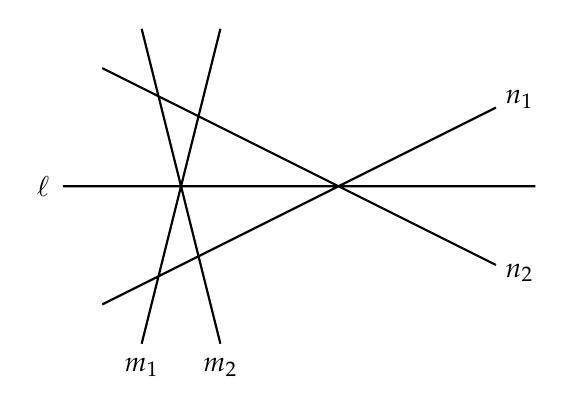
\begin{tikzpicture}
\draw[thick] (-3,0) -- (3,0) (-2,2) -- (-1,-2) (-2,-2) -- (-1,2) (2.5,1) -- (-2.5,-1.5) (2.5,-1) -- (-2.5,1.5);
\node at (-3.25,0) {$\ell$};
\node at (-2,-2.3) {$m_1$};
\node at (-1,-2.3) {$m_2$};
\node at (2.8,1.1) {$n_1$};
\node at (2.8,-1.1) {$n_2$};
\end{tikzpicture}
\caption{$\P^2$ minus five lines.}
\label{fig:cincolineas}
\end{figure}
Note that there is a line $\ell$ that passes through both triple points. the first one containing $m_1, m_2$, and the second one $n_1, n_2$. Using the pencil through $\ell \cap m_1 \cap m_2$, we can see $X$ as a subset of $\mathbb{C} \times (\P^1-\{3\text{ points}\}) \to \P^1 - \{3 \text{ points}\}$. But we are also removing $n_1$ and $n_2$, which removes two points from each fiber. This way, we get a map $\pi\colon X \to \P^1-\{3 \text{ points}\}$ from the pencil, such that each fiber is $\mathbb{C}-\{2 \text{ points}\}$. This shows that $X$ is Kobayashi hyperbolic, as claimed. 
\end{exm}

\section{Today}

Let us go back to Question \ref{que:hyperbolicity}, and see what is known today about hyperbolicity of hypersurfaces or their complements. See for instance Demailly for more details. 

For hypersurfaces, in 2002 Siu sketched a proof of generic hyperbolicity of hypersurfaces of high enough degree and completed it in 2015. This also has been proven by Demailly in 2020. Siu also showed that the complement of a general hypersurface is Brody hyperbolic, and Brotbek and Deng in 2019 proved that it is Kobayashi hyperbolic. See Voisin for a discussion on Siu's original proof.

The major problem is that their results have bad bounds for hyperbolicity: $(en)^{2n+2}/3$ from Demailly, and $(n+3)^{n+4}(n+2)^{n+4}$ from Brotbek--Deng. The lower bounds are essentially around $2n$, as we discussed today.

\chapter{Patrick (Mar 25): Curves on Calabi-Yau hypersurfaces}%

\textit{Note: these are the speaker's notes.}

First, we recall some basic definitions.

\begin{defn}
    Let $X$ be a smooth (or maybe with nice singularities prescribed by the MMP) variety. Then $X$ is \textit{Calabi-Yau} if $\omega_X = \mc{O}_X$.
\end{defn}

\begin{exm}
    By the adjunction formula, a degree $n+2$ hypersurface in $\P^{n+1}$ is Calabi-Yau. For some low dimensional examples, this means that elliptic curves, quartic surfaces, and quintic threefolds are Calabi-Yau.
\end{exm}

\begin{exm}
    Recall that if $f \colon Y \to X$ is a double cover branched along a divisor $D$, we have
    \[ K_Y = f^* \qty(K_X + \frac{1}{2} D). \]
    This implies that the double cover of $\P^2$ branched along a sextic is Calabi-Yau as is the double cover of $\P^3$ branched along an octic surface.
\end{exm}

\section{Rational curves on Calabi-Yau hypersurfaces}

We will now consider rational curves on Calabi-Yau hypersurfaces.

\begin{thm}[Clemens]
    Let $X$ be a general Calabi-Yau hypersurface of dimension $n \geq 2$. Then $X$ contains rational curves of arbitrarily large degree.
\end{thm}

For a quintic threefold, note that if we have $\P^1 \simeq C \subset X$, then the exact sequence
\[ 0 \to T_{C} \to T_{\P^3}|_C \to N_{C/X} \to 0 \]
tells us that $\deg N_{C/X} = -2$. Hirzebruch-Riemann-Roch for a smooth curve $C$ of genus $g$ says that
\[ \chi(C, \mc{E}) = \on{rk} \mc{E} (1-g) + c_1(\mc{E}), \]
and this gives us $\chi(N_{C/X}) = 0$ in our case. Generically, we expect (by upper semicontinuity of cohomology) that $h^0(N_{C/X}) = h^1(N_{C/X}) = 0$, and thus we expect
\[ N_{C/X} = \mc{O}(-1) \oplus \mc{O}(-1). \]
Actually, for any smooth rational curve $\P^1 \hookrightarrow X$ in a general quintic threefold, that is exactly the normal bundle by a result of Bin Wang in 2015. By basic deformation theory, we see that such $C$ are infinitesimally rigid. In fact, we can strengthen the previous theorem:

\begin{thm}
    Let $X$ be a quintic threefold. then $X$ has infinitely many infinitesimally rigid rational curves.
\end{thm}

On the flip side, we expect that there are not too many rational curves on a quintic threefold.

\begin{conj}[Clemens]
    Let $X$ be a general quintic threefold. Recall that by the Lefschetz hyperplane theorem, $H_2(X) = \Z$ is generated by the class of a line. Then for any $d > 0$, $X$ contains only finitely many rational curves of degree $d$.
\end{conj}

This conjecture is true in degrees $d \leq 11$ by a result of Cotterill in 2012. It also inspired the development of enumerative geometry, mirror symmetry, and many other ideas, but we will not discuss them here.

\begin{rmk}
    The conjecture is crucially supported by the fact that deformations of $C \simeq \P^1$ inside $X$ are unobstructed. On the other hand, if $Q$ is a quartic surface and $C \subset Q$ is a rational curve, then $N_{C/Q} = \mc{O}(-2)$, and because $h^1(N_{C/X}) = 1$, we see that deformations of $C$ in $Q$ are obstructed.
\end{rmk}

\begin{rmk}
    The Clemens conjecture is false if we let $X$ be a double cover of $\P^3$ ramified along an octic surface $S$. Consider lines $\ell$ such that $\ell \cap S = 2p_1 + 2 p_2 + 2 p_3 + p_4 + p_5$ as cycles. There is a $1$-dimensional family of such lines. If $\pi \colon X \to \P^3$ is the double cover, then $\pi^{-1}(\ell)$ is ramified over $\ell$ at $2$ points and is therefore rational. But this means we have a $1$-parameter family of rational curves in $X$ all of the same degree.
\end{rmk}

The remark is related to the following result:

\begin{prop}
    Let $X$ be a Calabi-Yau threefold and suppose that $X$ contains a smooth rational curve $C \simeq \P^1$ with normal bundle 
    \[ N_{C/X} \simeq \mc{O}(1) \oplus \mc{O}(1). \]
    Assume there exists a rational curve $C' \subset X$, a neighborhood $U \supset C \cup C'$, and an involution $i \colon U \to U$ such that
    \begin{enumerate}[(1)]
        \item The fixed locus of $i$ is a smooth hypersurface of $U$ that meets $C$ transversally;
        \item $i(C) = C' \neq C$.
    \end{enumerate}
    Then,
    \begin{enumerate}[(1)]
        \item If $i$ has at least one fixed point on $C$, then $X$ contains a one-parameter family of rational curves.
        \item If $i$ has two fixed points $p, p' \in C$ and the tangent directions to $C'$ at $p, p'$ are distinct in $\P(N_{C/X}) = C \times \P^1$, then $X$ is swept out by a two-parameter family of elliptic curves.
    \end{enumerate}
\end{prop}

To obtain this result, we need to choose a special octic surface. Let $\ell$ be a line in $\P^3$ and note that the map
\[ H^0(\P^3, \mc{O}_{\P^3}(8)) \to H^0(\P^1, \mc{O}_{\P^1}(8)) \]
is surjective (this is an exercise in Hartshorne). Now if we choose $f \in H^0(\P^1, \mc{O}(8))$ to vanish at three points with degrees $2,2,4$, then by a Bertini-type argument, the general octic surface $S$ living above $f$ is smooth. Now note that $\pi^{-1}(\ell)$ splits into two components because the local equation looks like
\[ y^2 = x^4 (x+1)^2 (x-1)^2, \]
and therefore the two components look like $y = \pm x^2 (x+1)(x-2)$. But now if we take $C, C'$ to be the two components and $i$ to exchange the two sheets, we see that both assumptions of the proposition are satisfied. We have already exhibited a one-parameter family of rational curves above, and later we will produce a two-parameter family  of elliptic curves.

\section{Sweeping out of hypersurfaces}

In this section we will discuss sweeping out of hypersurfaces by abelian varieties. This will roughly mean that a variety is covered by a generically finite morphism from a family of abelian varieties.

\begin{defn}
    Let $S$ be a quasiprojective variety and $f \colon \mc{Y} \to S$ be a smooth projective morphism of relative dimension $r$. Also let $X$ be a variety of dimension $n$. Then $X$ is \textit{rationally swept out} by members of $\mc{Y}$ if there exists a quasiprojective variety $B$ of dimension $n-r$, a morphism $B \to S$, and a dominant rational map $\mc{Y}_B \dashrightarrow X$.
\end{defn}

For example, we can consider when $S$ is a moduli space of varieties and $\mc{Y}$ is the universal family. Also, the definition of sweeping out is equivalent to the property that the union of the images of generically finite rational maps $Y_s \dashrightarrow X$ contains a Zariski open set of $X$.

The main result that Voisin proves about sweeping out of hypersurfaces by varieties is the following:

\begin{thm}[Voisin]
    Let $1 \leq r \leq n$ and $\gamma = \ceil{\frac{r-1}{2}}$. Let $S$ have dimension $C$ and $\mc{Y} \to S$ be a family of $r$-dimensional smooth projective varieties. Finally fix a positive integer $d$. Then, if the two inequalities
    \begin{enumerate}[(1)]
        \item $(d+1) r \geq 2n + C + 2$;
        \item $(\gamma + 1) d \geq 2n - r + 1 + C$
    \end{enumerate}
    hold, the very general hypersurface of degree $d$ in $\P^{n+1}$ is \textbf{not} swept out by members of the family $\mc{Y} \to S$.
\end{thm}

This result is a consequence of a Hodge-theoretic result. First, let $U \subset \abs{\mc{O}_{\P^{n+1}}(d)}$ be the open set parameterizing smooth hypersurfaces. Let $\rho \colon \mc{M} \to U$ be a morphism with $\mc{M}$ smooth and quasiprojective such that the corank of $\rho$ is constant and equal to $C$ and that the image of $\rho$ is stable under $GL_{n+2}$. Let $\mc{X}_U$ be the universal smooth hypersurface and $j \colon \mc{X}_{\mc{M}} \hookrightarrow \mc{M} \times \P^{n+1}$ be the natural closed immersion.

\begin{thm}[Nori]\leavevmode
    \begin{enumerate}[(1)]
        \item Assume that $(d+1)r \geq 2n+C+2$. Then the restriction
            \[ j^* \colon F^n H^{2n-r}(\mc{M} \times \P^{n+1}, \C) \to F^n H^{2n-r}(\mc{X}_{\mc{M}}, \C) \]
            is surjective.
        \item If $(\gamma + 1) d \geq 2n+1-r+C$, then the restriction
            \[ j^* \colon H^{2n-r-i}(\mc{M} \times \P^{n+1}, \C) \to H^{2n-r-i}(\mc{X}_{\mc{M}}, \C) \]
            is surjective for any $i \geq 1$.
    \end{enumerate}
\end{thm}

The proof of this is of course Hodge-theoretic and uses spectral sequences, and it is omitted here. Finally, we state a conjecture about the sweeping out of hypersurfaces by abelian varieties.

\begin{proof}[Proof of Voisin assuming Nori]
    Suppose that there is a $B$ of dimension $n-r$, maps $\rho \colon B \to S$ and $m \colon B \to U$, and a dominant $\phi \colon \mc{Y}_B \dashrightarrow \mc{X}_B$. But then if $f \colon \mc{Y}_B \to B$ and $\pi \colon \mc{X}_U \to U$ are the families, we have $\pi \circ \phi = m \circ f$.

    Now by shrinking $B$, we may assume that all $B_s$ for $s \in S$ are smooth and that the corank of $m_s \coloneqq m |_{B_S}$ is constant and $\leq C$. Now if $\mc{Y}_s \coloneqq f^{-1}(\mc{B}_s)$, write $\phi_s \coloneqq \phi |_{\mc{Y}_s}$. Therefore we have a rational map
    \[ \phi_s \colon \mc{Y}_s = Y_s \times \mc{B}_s \dashrightarrow \mc{X}_U \times_U \mc{B}_s \eqqcolon \mc{X}_s. \]
    But then the graph $\Gamma_{\phi_s} \subset Y_s \times \mc{B}_s \times_{\mc{B}_s} \mc{X}_s = Y_s \times \mc{X}_s$. This gives a cohomology class $\gamma_s \in H^{2n}(Y_s \times \mc{X}_s, \Q)$. Now Nori's theorem implies the class $\gamma_{s, r} \in H^r(Y_s, \Q) \otimes H^{2n-r}(\mc{X}_s, \Q)$ vanishes in 
    \[ H^r(Y_s, \Q)_{\mr{tr}} \otimes (H^{2n-r}(\mc{X}_s, \Q) / H^{2n-r}(\P^{n+1} \times \mc{B}_s, \Q)). \]

    Finally, returning to $\Gamma_{\phi} \subset \mc{Y}_B \times_U \mc{X}$, which has codimension $n$. If we fix $s \in S$, the class $[\Gamma_{\phi}] \in H^{2n}(\mc{Y}_B \times_U \mc{X}, \Q)$ restricts to $\gamma_s$. If we fix $u \in U$ and let $B_u \coloneqq m^{-1}(u)$. Then $\phi$ restricts to
    \[ \phi_u \colon \mc{Y}_u \eqqcolon \mc{Y} \times_S B_u \dashrightarrow X_u, \]
    which is dominant and generically finite on fibers. But now, a Hodge-theoretic argument tells us that
    \[ \phi_u^* \colon H^n(X_u, \Q)_{\mr{tr}} \to H^n(\mc{Y}_u, \Q) \]
    is injective and is in fact nonzero in $\Hom(H^n(X_u, \Q)_{\mr{tr}}, H^{n-r}(B_u, R^r f_* \Q_{\mr{tr}}))$. But now $[\Gamma_{\phi}]$ is nontrivial in $H^{2n}(\mc{X}_B, R^r f_* \Q_{\mr{tr}}) / H^{2n}(\mc{Y}_B \times \P^{n+1}, \Q)$, and so by a spectral sequence argument, $\gamma_{s,r}$ is nonzero, which is a contradiction.
\end{proof}

\begin{conj}[Lang]
    Let $X$ be not of general type. Then the union of the images of non-constant rational maps $\phi \colon A \dashrightarrow X$ from an abelian variety $A$ is $X$.
\end{conj}

Equivalently, this becomes:

\begin{conj}
    Let $X$ be a variety of Kodaira dimension $0 \leq \kappa(X) < \dim X$ (in particular, $X$ is not of general type). Then $X$ is rationally swept out by abelian varieties of dimension $r \geq 1$.
\end{conj}

Note that this conjecture is true when $X$ is a double cover of $\P^3$ branched along an octic surface $S$. Consider the two-parameter family of lines $\ell \subset \P^3$ such that
\[ \ell \cap S = 2 p_1 + 2 p_2 + p_3 + p_4 + p_5 + p_6. \]
Then the preimage of $\ell$ in $X$ is branched over $\ell \simeq \P^1$ at $4$ points, and therefore its normalization is an elliptic curve. But this implies that $X$ is swept out by a two-parameter family of elliptic curves.

\section{Sweeping out of Calabi-Yau hypersurfaces by abelian varieties}

\begin{thm}
    Let $X$ be a very general Calabi-Yau hypersurface in $\P^{n+1}$ (that is, of degree $d = n+2$). Then $X$ is \textbf{not} swept out by $r$-dimensional abelian varieties for any $r \geq 2$.
\end{thm}

\begin{proof}
    This boils down to checking some inequalities. First, recall that
    \[ \dim \mc{A}_r = \frac{r(r+1)}{2}. \]
    Then we need to check the two inequalities. The first is
    \[ (n+3)r \geq 2n + \frac{r(r+1)}{2} + 2, \]
    which is clearly true for $r \geq 2$ because
    \begin{align*}
        r\qty(n+3-\frac{r+1}{2}) \geq 2(n+1),
    \end{align*}
    which holds because $n + 3 - \frac{r+1}{2} + r \geq n+3$ and both $r \geq 2$ and $n+3-\frac{r+1}{2} \geq 3$. The second inequality is
    \[ (\gamma + 1)(n+2) \geq 2n - r + 1 + \frac{r(r+1)}{2}, \]
    and this holds for $r \geq 2$ by high school algebra (of the kind that I cannot bother to figure out).
\end{proof}

\begin{cor}
    If Lang's conjecture is true for a very general Calabi-Yau hypersurface $X$, then $X$ is swept out by elliptic curves.
\end{cor}

This will imply that $X$ has a uniruled divisor, but first we need the following lemma:

\begin{lem}
    Let $X$ be a very general Calabi-Yau hypersurface of dimension $\dim X \geq 2$. Then $X$ is not swept out by an isotrivial family of elliptic curves.
\end{lem}

\begin{lem}
    Suppose a variety $X$ is swept out by a non-isotrivial family of elliptic curves. Then $X$ has a uniruled divisor.
\end{lem}

\begin{proof}
    By assumption, we have a diagram
    \begin{equation*}
    \begin{tikzcd}
        \mc{K} \ar[dashrightarrow]{r}{\phi} \ar{d}{\pi} & X \\
        B,
    \end{tikzcd}
    \end{equation*}
    where $\mc{K} \to B$ is a family of elliptic curves. Now this is given by $B \to \mc{M}_{1,1}$, so we can choose a smooth projective model $B' \supset B$ and a smooth projective model $\mc{K}' \supset \mc{K}$. Now we can replace $\phi$ with an honest morphism
    \begin{equation*}
    \begin{tikzcd}
        \mc{K}' \ar{r}{\phi} \ar{d}{\pi} & X \\
        B'.
    \end{tikzcd}
    \end{equation*}
    But now the $j$-invariant map
    \[ j \colon B' \xrightarrow{\mc{K}'} \ol{\mc{M}}_{1,1} \to \P^1 \]
    (composing the defining map of $\mc{K}'$ with the coarse moduli space) is surjective. But now for $t \in \P^1$, consider the divisor
    \[ \mc{K}_t' \coloneqq (j \circ \pi)^{-1}(t). \]
    For a generic $t \in \P^1$, this is sent to a divisor of $X$, and in particular for any $t$, the image $\phi(\mc{K}_t')$ contains a divisor of $X$. But now if we take $t = \infty$, noting that an elliptic curve must degenerate to a union of rational curves, we see that any component of $\mc{K}_{\infty}'$ is uniruled, so we are done.
\end{proof}

\begin{cor}
    Clemens' conjecture and Lang's conjecture contradict each other.
\end{cor}

\chapter{Morena (Apr 01): Faltings and strong Lang-Vojta}%

We are interested in the cases where $k$ is either $\C, \ol{\Q}$, or a number field. We will always let $A, B$ be abelian varieties over $k$ and $X \subseteq A$ will be a closed subvariety of $A$. Finally, we will allow $\mc{L}$ to be a symmetric ample line bundle on $A$. Finally, we will consider the notions of being pseudo-(Brody, Kobayashi, groupless, Mordellic).

Recall that $X/\ol{Q}$ is Mordellic mod $\Delta$ if there exists a model of $X$ over $\Q$ such that $X_K(K) \setminus \Delta$ is finite for all number fields $K/\Q$. Also recall that $X$ is groupless mod $\Delta$ if any nonconstant $f \colon B \dashrightarrow X$ satisfies $f(B) \subseteq \Delta$.

\begin{rmk}
    Considering rational maps $B \dashrightarrow X$ is the same as considering morphisms $B \to X$ and $\mathbb{G}_m \to X$. To see this, note that a map from $\mathbb{G}_m$ extends to a map from $\P^1$, so we can consider a double cover $E \to \P^1 \to X$ defined by $\mc{O}_E(-2)$. Then we require a lemma:
\end{rmk}

\begin{lem}[Javanpeykar-Kamenove]
    If $X$ is proper and has no rational curves, any rational map $B \dashrightarrow X$ extends to a morphism $B \to X$.
\end{lem}

\section{Strong Lang-Vojta}

Now we will state the strongest Lang-Vojta conjecture.

\begin{conj}[Strongest Lang-Vojta]
    Let $X/K$ be a projective variety. Then
    \begin{enumerate}[(1)]
        \item If $K = \ol{Q}$, then $X$ is groupless mod $\Delta$ if and only if it is Mordellic mod $\Delta$;
        \item $X$ is of general type if and only if
            \[ \Delta^{\mr{gr}} = \bigcap_{X \text{ groupless mod }\Delta} \Delta \neq X; \]
        \item If $K = \C$, then $X$ is groupless mod $\Delta$ if and only if $X$ is Brody mod $\Delta$ if and only if $X$ is Kobayashi mod $\Delta$.
    \end{enumerate}
\end{conj}

In general, we know that $\Delta^{\mr{gr}} \subset \Delta^{\mr{Mor}}$ and $\Delta^{\mr{gr}} \subseteq \Delta^{\mr{Br}} \subseteq \Delta^{\mr{Kob}}$.

\begin{defn}
    Define the \textit{special locus} of $X$ to be
    \[ \mr{Sp}(X) = \bigcup_{x + B \subseteq X} x + B \subseteq X. \]
\end{defn}

We hope that this is a closed subscheme of $X$. Now consider $X \subseteq A$ to be a closed subvariety.

\begin{thm}[Kawamata]
    There exists a closed subscheme $Z \subseteq X$ such that for all $Z_i \subseteq Z$, there exists $B_i \subseteq A$ such that $Z_i = \qty{x \in X \mid x + B_i \subseteq X}$. Moreover, if any $B \subseteq A$ satisfies $x + B \subseteq X$, then $X + B \subseteq Z$, then $Z = \mr{Sp}(X)$.
\end{thm}

\begin{rmk}
    The formation of $Z$ commutes with base change and works for any $K$, but maybe we need to take a finite extension of $K$.
\end{rmk}

\begin{proof}
    Define the map
    \[ \alpha_m \colon X^m \to A^{m-1} \qquad (x_1, \ldots, x_m) \mapsto (2 x_1 - x_2, 2 x_2 - x_3, \ldots, 2 x_{m-1} - x_m). \]
    Then define $Y_m$ to be the pullback in the diagram
    \begin{equation*}
    \begin{tikzcd}
        Y_m \ar{r} \ar{d} & X^m \ar{d}{\alpha_m} \\
        X \ar{r}{\Delta} & A^{m-1}.
    \end{tikzcd}
    \end{equation*}
    In particular, we see that
    \[ Y_m = \qty{(x, a) \in X \times A \mid x + 2^i a \in X \text{ for all }0 \leq i \leq m} \subseteq X \times A. \]
    Now we consider $Y_{m+1} \subseteq Y_m$, so define $Y_{\infty} = \bigcap Y_m$. In particular, we have
    \[ Y_{\infty} = \qty{(x, a) \in X \times A \mid x + 2^i a \in X \text{ for all } i \geq 0}. \]
    We know $Y_{\infty} \subseteq X \times A$ and now consider $W \subseteq (Y_{\infty})_x = Y_{\infty} \cap \qty{x} \times A$.

    First, if $\dim W > 0$, there exists $x_W + B = W$. In addition, the set of all $B$ such that $x_W + B = W \subseteq (Y_{\infty})_x$ is finite. When $x = 0$, we have $2^n \colon W \to W$, and if we consider
    \[ W \xrightarrow{2^n} W \hookrightarrow A, \]
    we see that $\deg_{(i \circ 2^n)^* \mc{L}} (W) = (2^n)^{2 \dim W} \deg (W)$. This tells us that
    \[ \deg_{i^* \mc{L}}(2^n W) = \frac{(i^* \mc{L})^{\dim W} 2^n_* [W]}{\deg (2^n W / W)} = \frac{2^{2n\dim W} \deg W}{\# \qty{(2^n)^{-1} (\xi_W)}} \]
    by the projection formula.

    Then $(2^n)^{-1}(\xi_W) = \qty{g \in A[2^n] \mid g + \xi_W \in W}$, so if we define $G = \qty{g \in A, g + W \subseteq W}$, we note that
    \[ \# (2^n)^{-1} (\xi_W) = \# G[2^n] = (2^n)^{\dim G}. \]
    But then because $\deg (2^n (W))$ is bounded, $\dim G = \dim W > 0$, so it is enough to consider $G_{\mr{red}}^0 = B$.

    Now we will use Noetherian induction and reducing to the flat locus, and finally Stein factorization. Now consider $Y_{\infty} \to X$, so let $U \subseteq Y_{\infty}$ be the flat locus. Because $Y_{\infty} \setminus U_{\infty}$ has lower dimension, we may assume that $Y_{\infty}$ is flat over $X$. Second, by taking irreducible components, we may assume $Y_{\infty}$ is irreducible. Third, by taking Stein factorization, we may assume that the fibers of $Y \to X$ are geometrically connected. After these reductions, we have a map
    \[ X \to \mr{Hilb}_{A/k}. \]
    If this map is nonconstant, we have uncountably many $B \subseteq A$ translating to $Y_{\infty}$, but this contradicts the fact that there are only countably many $B \subseteq A$. Finally, we define
    \[ Z = \qty{x \in X \mid \dim_x (Y_{\infty})_x > 0}. \qedhere \]
\end{proof}

There is a relationship between $\mr{Sp}(X)$ and $\Delta^{\mr{gr}}$.

\begin{rmk}
    Let $K$ be a number field. Then $\mr{Sp}(X) = \Delta^{\mr{gr}}$. To see this, consider $f \colon B \to X \hookrightarrow A$. Then the image of $f$ is $x + B$, so it lives in the special locus.
\end{rmk}

\begin{cor}
    The strong Lang-Vojta conjecture is true for $X \subseteq A/K$.
\end{cor}

By Bloch's theorem, we note that $X$ being of general type over $\C$ is equivalent to $\mr{Sp}(X) \neq X$. Because $\mr{Sp}(X)$ is stable under base extension, we can check both being of general type and the condition on $\Delta^{\mr{gr}}$ by taking the base change to $\C$.

\section{Special locus and the Mordellic locus}

\begin{thm}
    Let $X \subseteq A / \ol{Q}$. Then $X$ is Mordellic mod $\mr{Sp}(X)$.
\end{thm}

\begin{proof}
    Consider $(x_1, \ldots, x_m) \in (X \setminus \mr{Sp}(X))(K)$ such that 
    \begin{itemize}
        \item $h(x_1)$ and $\frac{h(x_i)}{h(x_{i-1})}$ are large, where $h(y) = \frac{\log H_K(y)}{[K:\Q]}$;
        \item $A(K) = \Z^{\mr{rk}} \oplus \text{finite}$ and $x_i$ are not torsion;
        \item After passing to $A(k) \otimes \R$, the angles $\frac{\ev{x_i, x_j}}{\norm{x_i} \norm{x_j}}$ are small.
    \end{itemize}
    Our goal is to define a chain of $Y^{(j)} = Y_1^{(j)} \times \cdots \times Y_m^{(j)} \subseteq X^m$ such that $(x_1, \ldots, x_m) \in Y^{(j)}$ but the dimensions are strictly decreasing. We will use a black box of Siegel's lemma and a product theorem of Faltings.

    Now consider $\mc{L}$ a symmetric ample line bundle and define
    \[ \mc{L}(s) = \sum (s_i \mr{pr}_i - s_{i-1} \mr{pr}_{i-1})^* \mc{L}, \]
    where $s \in \Q^r$. Also, define $H(s) = \sum s_i^2 \mr{pr}_i^* \mc{L}$. Note that $\mc{L}(s)^d \cdot Y$ and $H(s)^d \cdot Y$ have the same order of growth, where $Y = Y_1 \times \cdots \times Y_m \subseteq X^m$ and $\dim (Y_i) = d_i$.

    Now assume $m \gg 0$. There exists $\ep > 0$ such that for all $Y = Y_1 \times \cdots \times Y_m$ for $Y_i \not\subseteq \mr{Sp}(X)$ and for all $s = (s_1, \ldots, s_r)$ there exists $c(Y, s)$ such that
    \[ \dim H^0(Y, (\mc{L}(s) - \ep H(s))^{\otimes m'}) \geq c(Y, S) \dim H^0(Y, H(s)^{\otimes m'}). \]
    This is proved roughly by noting that $\alpha_m$ is quasi-finite on $(X \setminus \mr{Sp}(X))^m$ for large enough $m$. Thus we can define 
    \[ W_m = \qty{x \in A^{m-1} \mid \dim \alpha_m |_{(X \setminus \mr{Sp}(X))^m}} = d(m) > 0. \]
    Then if $m \gg 0$ such that the above holds, then $\alpha_m^* (H(S)) - \ep H(s)$ is generated over $(X \setminus \mr{Sp}(m))^m$ by global sections defined on $X^m$. If a curve $C \subseteq X^m$ meets $(X \setminus \mr{Sp}(X))^m$, then
     \[ \deg (\alpha_m^* H(s) - \ep H(s) \cdot C) \geq 0. \]

     Next, we show that $\alpha_m^* H(s) = \mc{L}(s)$ for $s_i = 2^{m-i}$. Here, we use a theorem of Burnof such that if $H$ is ample and $\mc{L}^{\dim Y} \cdot Y \geq 0$, and there exists $E \subseteq X$ such that for all $C \subseteq X$ not contained in $E$, $\mc{L} C \geq \eta \cdot H \cdot C$. This implies that
     \[ \mc{L}^{\dim Y} \cdot Y \geq \eta^d H^{\dim Y} \cdot Y \]
     and that
    \[ (\alpha_m^* H(s) + \delta H(s))^d \cdot Y \geq \ep^d H(s)^d \cdot Y \]
    for our particular choice of $s$, and thus is true for all $s = (s_1, \ldots, s_r)$. Finally, we intersect with hyperplanes and bound the dimension.
\end{proof}

\begin{thm}[Faltings]
    There exist finitely many translates $x_i + B_i \subseteq X$ where $x_i \in X(K)$ and $B_i$ are defined over $K$ such that $X(k) \subseteq \bigcup x_i + B_i$. 
\end{thm}

\chapter{Kuan-Wen (Apr 08): Finiteness of morphisms to algebraically hyperbolic varieties}%

\section{Overview}

Our main goal is the following result:

\begin{thm}\label{thm:surj}
    Let $X$ be a projective algebraically hyperbolic scheme. Then
    \begin{enumerate}[(1)]
        \item If $Y$ is a projective variety, then $\abs{\mr{Sur}(Y, X)} < \infty$;
        \item $\mr{Sur}(X, X) = \Aut(X)$ and $\abs{\Aut}(X) < \infty$.
    \end{enumerate}
\end{thm}


Historically, we have the following results.
\begin{thm}
    Let $C_1, C_2$ be curves with $g(C_i) \geq 2$. Then $\abs{\Hom^{\mr{nc}}(C_1, C_2)} < \infty$ and if we fix $C_1$, only finitely many $C_2$ admit nonconstant morphisms.
\end{thm}

\begin{thm}[Kobayashi-Ochion]
    The conditions in Theorem~\ref{thm:surj} are satisfied for varieties of general type.
\end{thm}

\begin{thm}[Naguchi]
    Theorem~\ref{thm:surj} holds for Brody hyperbolic varieties.
\end{thm}

\begin{thm}[Javanpeykar-Xie]
    Theorem~\ref{thm:surj} holds for pseudo-algebraically hyperbolic varieties.
\end{thm}

\begin{thm}[Matsumura]
    If $X$ is of general type, then there are only finitely many dominant rational maps $X \dashrightarrow X$.
\end{thm}

\begin{defn}
    Let $X$ be a projective variety. Then $X$ is \textit{bounded} if for any normal projective variety $Y$, the scheme
    \[ \ul{\Hom}_k(Y, X) \subseteq \on{Hilb}_k(Y \times X) \]
    is of finite type.
\end{defn}

Also recall the definitions of algebraic hyperbolicity and grouplessness.

\begin{defn}
    A projective variety $X$ is \textit{pure} if there exist no nonconstant maps $\P^1 \to X$.
\end{defn}

\begin{prop}
    Algebraic hyperbolicity implies boundedness implies grouplessness implies purity.
\end{prop}

\begin{proof}
    Let $f \in \Hom(Y, X)$ and let $H, D$ be ample divisors on $Y, X$, respectively. Then fix a sufficiently large constant $a$. We know that
    \[ \int_{\Gamma_f} c_1(\on{pr}_1^* a H + \on{pr}_2^* D)^m = \int_Y c_1(\mc{O}_Y(aH + f^* D))^m. \]
    Therefore we need to bound $(aH)^{m-1} (f^* D)$. Then by the numerical criterion for bigness, which says that for $X$ projective and $D, Z$ nef, if $D^m > m (D^{m-1} E)$, then $D-E$ is big, because $(aH)^m > m (aH)^{m-1} (f^* D)$, $aH - f^* D$ is big. Then
    \[ (aH - f^* D) (aH)^{m-1-i} (f^* D)^i \geq 0, \]
    and therefore
    \[ a^m H^m \geq a^{m-1} H^{m-1} f^* D \geq \cdots \geq (f^* D)^m \geq 0, \]
    so $\int_Y c_1(\mc{O}_Y(aH + f^* D))^m \geq 2^m a^m H^m$.

    Now if $X$ is bounded, if $f_m \colon C \subseteq A \xrightarrow{m_A} A \xrightarrow{f} X$, we know that $\deg_C f_m^* L = m^2 \deg_C f^* L$, which implies that $f^* L = 0$, so $f$ is constant. Finally, if there is a nonconstant map $\P^1 \to X$, there is a nonconstant $E \to \P^1 \to X$.
\end{proof}

\begin{cor}
    Let $X$ be a smooth projective variety with $\Omega_X^1$ ample and $Y$ be a normal projective variety. Then $\abs{\Hom^{\mr{nc}}(Y, X)} < \infty$.
\end{cor}

To see this, note that $T_{\Hom(Y, X), f} = \Hom(f^* \Omega_X^1 \mc{O}_Y) = H^0(Y, f^* T_X) = 0$.

\begin{lem}
    Suppose $X$ is groupless and let $G$ be a connected algebraic group scheme. Then any map $G \to X$ is constant.
\end{lem}

\begin{cor}
    Suppose $X$ is groupless. Then $\Aut^0(X) = \qty{1}$. If $X$ is bounded, then $\abs{\Aut(X)} < \infty$.
\end{cor}

\begin{proof}[Proof of lemma]
    By the Chevalley structure theorem, there is an exact sequence
    \[ 0 \to H \to G \to A \to 0, \]
    where $H$ is a linear group and $A$ is an abelian variety. We only need to consider linear groups. Let $U \subseteq H$ be the unipotent radical. Because there are no nonconstant maps $\P^1 \to X$, there are no morphisms from $\mathbb{G}_m, \mathbb{G}_a$. This reduces to the case of a reductive group $H/U$, but reductive groups are covered by Borels, so we are done.
\end{proof}

\begin{rmk}
    Let $X$ be a pure variety and $Y$ be smooth. Then any rational map $Y \dashrightarrow X$ is everywhere defined, so $\ul{\Hom}_k^P(Y, X)$ is projective.
\end{rmk}

Now let $\mc{P}$ denote the properties of being Kobayashi hyperbolic, algebraically hyperbolic, bounded, groupless, or pure.

\begin{prop}
    Let $X$ be projective with $\mc{P}$ and $Y$ be normal projective. Then $\ul{\Hom}_k^P(Y, X)$ is projective with $\mc{P}$ with dimension $\dim \leq \dim X$.
\end{prop}

\begin{proof}
    If $f \colon Y \to X$ is finite, then if $X$ has $\mc{P}$, so does $Y$. Now let $\wt{Y} \to Y$ be the desingularization. By a rigidity lemma, $\ul{\Hom}_k(Y, X) \hookrightarrow \ul{\Hom}_k(\wt{Y}, X)$ as connected components. Therefore, we can assume $Y$ is smooth.

    Now if we fix $y \in Y$, the map $\ul{\Hom}_k^p(Y, X) \to X$ given by $f \mapsto f(y)$ is finite. To see this, if $H \subseteq \qty{f(y) = x}$ is a connected component, consider the map $H \times Y \to X$ gievn by $(f, y') \mapsto f(y')$. Then $H \times \qty{y} \to \qty{x}$, so $H$ is a singleton.
\end{proof}

\section{Proof of the main theorem}

We will first prove the following:

\begin{thm}[Hwang-Kebokus-Peternell]
    Let $X, Y$ be normal projective varieties and suppose that $Y$ is not uniruled. Also suppose that $f \in \on{Sur}(X, Y)$. Then there exists a factorization
    \begin{equation*}
    \begin{tikzcd}
        X \ar{rr}{f} \ar[swap]{dr}{\alpha} && Y \\
        & Z \ar[swap]{ur}{\beta}
    \end{tikzcd}
    \end{equation*}
    such that $\beta$ is finite and \'etale outside of the singular locus of $Y$ and the morphism
    \[ \Aut^0(Z) \to \ul{\Hom}(X, Y) \qquad g \mapsto \beta \circ g \circ \alpha \]
    is \'etale and surjective onto the component containing $f$.
\end{thm}

\begin{rmk}
    Note that $Z$ is not uniruled, so $\Aut^0(Z)$ is an abelian variety, so the deformations of $f$ are unobstructed.
\end{rmk}

\begin{cor}
    Let $X$ be projective and groupless with $Y$ normal. Then $\dim \on{Sur}(Y, X) = 0$.
\end{cor}

\begin{proof}
    Factor $f \colon Y \to X$ into $Y \xrightarrow{\alpha} Z \xrightarrow{\beta} X$ with $\qty{1} = \Aut^0(Z) \twoheadrightarrow \Hom_f(Y, X)$.
\end{proof}

\begin{cor}
    Let $X$ be projective and bounded and $Y$ be projective. Then there are only finitely many dominant rational maps $Y \dashrightarrow X$.
\end{cor}

The key ingredient in the proof of the theorem is the following:
\begin{thm}[Miyaoka]
    Let $X$ be projective and not uniruled. Then $\Omega_X^1$ is generically semipositive. This means that for a general complete intersection curve $C$ and $\Omega^1_X |_C \twoheadrightarrow$, $\deg \mc{F} \geq 0$.
\end{thm}

For simplicity, assume that $X$ and $Y$ are smooth and $f \colon X \to Y$ is finite and surjective. In particular, $f$ is flat. Then we have the trace map $\mc{O}_Y \hookrightarrow f_* \mc{O}_X$, so $f_* \mc{O}_X = \mc{O}_Y \oplus \mc{E}^*$, where $\mc{E}^*$ is a vector bundle. Our goal is to find a subbundle $\mc{F} \subseteq \mc{E}^*$ such that
\begin{enumerate}[(1)]
    \item $\mc{O}_Y \oplus \mc{F}$ is an $\mc{O}_Y$-algebra. Then we can define $Z = \Spec \mc{O}_Y \oplus \mc{F}$.
    \item For any complete intersection curve $C$, $\deg \mc{F} |_C = 0$.
\end{enumerate}
Here, note that if $f \colon C_1 \to C_2$ is a finite morphism between smooth curves, then $\deg (f_* \omega_{C_1 / C_2}) = \frac{1}{{2}} \deg \mc{R}$.

Our candidate for $\mc{F}$ comes from the Harder-Narasimhan filtration. Set $\mc{E} = (\mc{E}^*)^* = f_* \omega_{X/Y} / \mc{O}_Y$. Then
\[ HN^{(\ell-1)} (\mc{E}) \subsetneq HN^{(\ell)}(\mc{E}) = \mc{E}. \]
We can now set
\[ \mc{F} = (\mc{E} / HN^{(\ell-1)}(\mc{E}))^*. \]
Also note that if $Y$ is nonsingular, $C$ is a general complete intersection curve, and $V$ is semistable on $Y$, then $V|_C$ is semistable. Therefore the restriction of the Harder-Narasimhan filtration is the Harder-Narasimhan filtration of the restriction.

\begin{lem}
    Assume that the morphism
    \[ T_{\Aut(Y), 1} = \Hom(\Omega^1_Y, \mc{O}_Y) \to \Hom(\Omega^1_Y, f_* \mc{O}_X) = \Hom(f^* \Omega_Y^1, \mc{O}_X) = T_{\Hom(Y, X), f} \]
    is not surjective. Then $\mc{E}\_C$ is nef but not ample for a general complete intersection curve $C$.
\end{lem}

\begin{proof}
    Recall that $\mc{E} = f_* \omega_{X/Y} / \mc{O}_Y$. By a result of Viehweg, $f_* \omega_{X/Y}|_C$ is nef, so $\mc{E}$ is also nef. But now
    \[ \Hom(f^* \Omega_Y, \mc{O}_X) = H^0(X, f^* T_Y) = H^0(Y, TY) \oplus H^0(Y, \mc{E}^* \otimes T_Y), \]
    because $f_* f^* T_Y = T_Y \oplus \mc{E}^* \otimes T_Y$. Now we now that $\Omega_Y^1 \twoheadrightarrow \mc{F}^*$, so $\deg \mc{F}^* |_C \geq 0$. However, because $\mc{E} \twoheadrightarrow \mc{F}$, if $\mc{E}$ is ample, then $\mc{F}$ is also ample, so $\deg (\mc{F}|_C) > 0$, which is a contradiction.
\end{proof}

\begin{lem}
    Let $C$ be a smooth curve and suppose that $E$ is nef but not ample. Then $HN^{(\ell-1)}(E)$ is the maximal ample subbundle of $E$ and has minimal rank with degree $\deg E$.
\end{lem}

\begin{proof}[Sketch of proof]
    We only need Hartshorne's characterization of ample vector bundles on curves. On $C$, $V$ is ample (nef) if and only if for all $V \twoheadrightarrow V'$, $\deg V' > 0$ (or $\geq 0$). First, any semistable bundle of positive degree is ample. Also, any bundle of nonnegative degree containing no ample subbundle is semistable.

    Then $HN^{(1)}$ is semistable and has positive degree, so it must be ample. If $V$ is the maximal ample subbundle of minimal rank with degree $\deg E$, $HN^{(1)} \subseteq E$. Thus $\deg (HN^{(k)}) = \deg (E)$. If this is ample, then $HN^{(k)} \subseteq V$ and $HN^{(k)} \supseteq V$ by minimality. Thus $k = \ell - 1$.
\end{proof}

Now we need to show that $\mc{O}_Y \oplus \mc{F}$ is an $\mc{O}_Y$-algebra. Here, we need to show that the map
\[ \ol{\mu}_C \colon (\mc{O}_C \oplus \mc{F}_C) \otimes (\mc{O}_C \oplus \mc{F}_C) \to (\mc{O}_C \oplus \mc{E}_C) / (\mc{O}_c \oplus \mc{F}_C) = HN^{(\ell-1)}(\mc{E})^* \]
is the zero map. But here, $V$ is def and has degree $0$, so $V^*$ is nef. 

Now we can factor
\begin{equation*}
\begin{tikzcd}
    X \ar{rr} \ar{dr} && Y \\
    & Z \ar{ur}
\end{tikzcd}
\end{equation*}
such that $T_{\Aut(Z), 1} \to T_{\Hom(X, Y), f}$ is an isomorphism. This uses the fact that if $g \colon A \to B$ is a morphism with $A$ smooth projective and $B$ connected such that $T_A \to g^* T_B$ is an isomorphism, then $g$ is \'etale and surjective.

In the general case, if 
\begin{equation*}
\begin{tikzcd}
    X \ar{rr}{f} \ar[swap]{dr}{f_* \mc{O}_X} & & Y \\
    & Z \ar[swap]{ur}{\text{finite}}
\end{tikzcd}
\end{equation*}
is the Stein factorization, we need to check that $\Hom_f(X, Y) = \Hom_f(Z, Y)$. If $f \colon X \to Y$ is finite, let $Y_0$ be the smooth locus of $Y$ with $f(\on{Sing}(X))$ removed. Then the singularities have codimension $2$, so if $C$ is a general complete intersection curve, $C \subseteq Y_0$. In addition, $\ul{\Hom}(f^* \Omega_Y, \mc{O}_X)$ is reflexive, so
\[ \Hom(f^* \Omega_Y, \mc{O}_X) = \Hom(f^* \Omega_{Y_0}, \mc{O}_{X_0}). \]
Taking the factorization $X_0 \to Z_0 \to Y_0$, because $\pi_1(Y) = \pi_1(Y_0)$, we can compactify this to $X \to Z \to Y$.

\chapter{Kevin (Apr 15): Uniformity of rational points}%

\section{Introduction}

Recall the statement of Faltings' theorem:
\begin{thm}[Faltings]
    If $X$ is a curve of genus $g \geq 2$ over a number field $K$, then $X(K)$ is a finite set.
\end{thm}

There are conjectured generalizations of this in higher dimension, due to Lang.
\begin{conj}[Weak Lang]
    Let $X$ be a variety of general type over a number field $K$. Then $X(K)$ is not Zariski-dense in $X$.
\end{conj}

\begin{conj}[Strong Lang]
    Let $X$ be a variety of general type over a number field $K$. Then there exists a proper closed subvariety $Y \subset X$ such such that for all finite extensions $L/K$, the set $X(L) \setminus Y(L)$ is finite.
\end{conj}

\begin{conj}[Geometric Lang]
    If $X$ is a variety of general type, then the union of all irreducible, positive-dimensional subvarieties not of general type is a proper closed subvariety of $X$.
\end{conj}

Note that weak Lang and geometric Lang imply strong Lang. Strong Lang is known for subvarieties of abelian varieties and geometric Lang is known for surfaces with $c_1^2 > c_2$. Now we will state the main theorems of the talk.

\begin{thm}[Uniform bound]
    Assume the weak Lang conjecture. Then for a fixed number field and a fixed genus $g$, there exists a uniform bound $B(K, g)$ on the number of $K$-points of genus $g$ curves over $K$.
\end{thm}

\begin{thm}[Uniform generic bound]
    Assume the strong Lang conjecture. Then for all $g \geq 2$, there exists $N(g)$ such that for all number fields $K$, there are finitely many isomorphism classes of genus $g$ curves over $K$ that have more than $N(g)$ points.
\end{thm}

The main geometric ingredient to these results is the following:
\begin{thm}[Correlation theorem]
    Let $X \to B$ be a proper morphism of integral varieties over $K$ with generic fiber a curve of genus $\geq 2$. Then for all $n \gg 0$, the fiber product 
    \[ X_B^n \coloneqq \underbrace{X \times_B \cdots \times_B X}_{n} \]
    admits a dominant rational map to a variety of general type.
\end{thm}

\section{Proof of uniform bound asssuming correlation}

\begin{lem}
    Let $X \to B$ be a flat family of curves. Then there exists a nonempty open $U_0 \subset B$ and $N \in \Z$ such that for all $b \in U_0(K)$, $\# X_b(K) \leq N$.
\end{lem}

\begin{proof}
    By correlation, there exists $n$ such that there exists a dominant $h \colon X_B^n \dashrightarrow W$ to a variety $W$ of of general type. Then by weak Lang, there exists an open $W' \subset W$ containing no $K$-points. Finally, let $U \subset X_B^n$ be the largest open subset such that $h$ is defined on $U$ and $h(U) \subset W'$. Then
    \[ Z \coloneqq X_B^n \setminus U \]
    contains all of the $K$-points of $X_B^n$.

    Now for $1 \leq j \leq n$, let $\pi_j \colon X_B^j \to X_B^{j-1}$ be the projection forgetting the last coordinate. Then let $Z_n$ be the subset $Z \subset X_B^n$ defined above. Going from $j = n-1$ to $j = 0$, let $Z_j \subset X_B^j$ be the largest closed subset such that $\pi_{j+1}^{-1}(Z_j) \subset Z_{j+1}$. Note $Z_j \neq X_B^j$ because $Z \neq X_B^n$, so let $U_j \coloneqq X_B^j \setminus Z_j$. The restriction 
    \[ \pi_j \colon \pi_j^{-1}(U_{j-1}) \cap Z_j \to U_{j-1} \] 
    is finite. Now let $d_j$ be the largest degree of a fiber of $\pi_j |_{\pi_j^{-1}(U_{j-1}) \cap Z_j}$.

    Consider $U_0 \subset B$, where $b \in U_0(K)$. We want to show that $X_b(K) \leq \max d_j$. Let $j$ be the smallest integer such that all $K$-points of $X_B^j$ lying above $b$ are contained in $Z_j$. This $j$ exists because $U_n$ contains no $K$-points. Then there exists $u \in U_{j-1}(K)$ mapping to $b$. The fiber $X_u = \pi_j^{-1}(u)$ is isomorphic to $X_b$, and thus $\# X_b(K) = \# X_u(K) \leq d_j$.
\end{proof}

Now we want to construct a family with every genus $g$ curve, and here we will use the Hilbert scheme and $n$-canonical embeddings. If $C$ is a curve a genus $g \geq 2$, $K_X^n$ is very ample for all $n \geq 3$. For example, take $n = 10$, $h(t) = dt - g + 1$, $d = 10(2g-2)$, and $r = d-g$. Then consider the Hilbert scheme $\on{Hilb}(\P^r, h(t))$, which contains every genus $g$ curve. Then write $H_g \subset \on{Hilb}(\P^r, h(t))$ for the locally closed, smooth, and irreducible locus of smooth curves. Write $B = H_g$ and $X \to B$ be the pullback of the universal closed subscheme from $\on{Hilb}(\P^r, h(t))$.

Now induct downwards on the dimension of $B$,use the lemma to obtain open subsets of $B$, and then by Noetherian induction, we obtain a uniform bound.

\section{The correlation theorem}

We will consider two examples of extreme cases: isotrivial families and families with maximal variation of moduli. First, consider the family
\[ X = \qty{y^2 = t f(x)} \xrightarrow{t} B = \A^1 \]
for a fixed degree $6$ polynomial $6$. Note all smooth geometric fibers are isomorphic. Note that the case $n=1$ fails because $X$ is rational. When $n = 2$, our family becomes
\[ X_B^2 = \qty{y^2 = tf(x), v^2 = tf(u)}. \]
This in fact has a morphism to a variety of general type. Consider the diagram
\begin{equation*}
\begin{tikzcd}
    X_B^2 \ar[dashrightarrow]{r}{\text{forget }t} \ar[dashrightarrow]{d}{(x,u)} & V \ar{dl} \\
    \P^1 \times \P^1,
\end{tikzcd}
\end{equation*}
where $V \to \P^1 \times \P^1$ is a double cover branched along $f(x) f(u) = 0$, so $K_V = \pi^* \mc{O}_{\P^1 \times \P^1}(1,1)$ is big.

We will now consider a family with maximal variation of moduli. Consider the family
\[ X = \qty{f(x,y) + t g(x,y) = 0} \xrightarrow{t} B = \P^1, \]
where $f, g$ are general quartics. Note that $X$ is rational, so we consider $Y = X_B^2$, which will be of general type. Note that
\[ X_B^2 = \qty{f(x,y)+tg(x,y) = 0, f(u,v)+t g(u,v) = 0} \subset \P^1 \times \P^2 \times \P^2. \]
This is complete intersection of two hypersurfaces with degrees $(1,4,0)$ and $(1,0,4)$, so by the adjunction formula,
\begin{align*}
    \omega_Y &\cong \omega_{\P^1 \times \P^2 \times \P^2}|_Y \otimes \mc{O}_{Y(1,4,0)} \otimes \mc{O}_{Y}(1,0,4) \\
    &\cong \mc{O}_Y(-2, -3, -3) \otimes \mc{O}_Y(1,4,0) \otimes \mc{O}_Y(1,0,4) \\
    &\cong \mc{O}_Y(0,1,1),
\end{align*}
which is big. It remains to deal with the singularities of $Y$, which are in fact ordinary double points for a sufficiently general pencil. Then ordinary double point singularities are canonical, which means that for $\pi\colon \wt{Y} \to Y$, $\pi^* K_Y = K_{\wt{Y}} \otimes \mc{O}_{\wt{Y}}(-D)$, where $D$ is effective. In fact, any resolution $\wt{Y}$ is of general type, so $Y$ is of general type.

\chapter{Akash (Apr 22): The product theorem}%

\section{Introduction}

Let $k$ be a field of characteristic $0$. Then let $P \coloneqq \P^{n_1} \times \cdots \times \P^{n_m}$ and $\mc{L}_i = \mr{pr}_i^* (\mc{O}(1))$. Then any $F \in H^0(P, \mc{L}_1^{\otimes d_1} \otimes \cdots \otimes \mc{L}_m^{\otimes d_m})$ is a multi-homogeneous polynomial of degree $(d_1, \ldots, d_m)$. We can also consider differential operators of multi-degree $(r_1, \ldots, r_m)$. Write
\[ L = \prod \pdv[a_{ij}]{x_{ij}}, \qquad \sum_j a_{ij} = r_i. \]
Then define the weighted degree of $L$ to be $\frac{r_1}{d_1} + \cdots + \frac{r_m}{d_m}$.

\begin{exm}
    Consider $\P^1_{x_0,x_1} \times \P^1_{y_0, y_1}$ and write
    \[ L = \pdv[3]{x_0} \pdv{x_1} \pdv[4]{y_1}, \]
    which has degree $(4,4)$. Then if $F = x_0^3 x_1^2 y_1^3 y_0^3$, the weighted degree is $\frac{4}{5} + \frac{4}{6}$.
\end{exm}

Now we define the index $i(x,F)$ at a point $x \in P$ to be the largest $\sigma$ such that $L(f)(x) = 0$ for all $L$ of weighted degree $\sum \frac{r_i}{d_i} \leq \sigma$. Then define the closed subscheme 
\[ Z_{\sigma} = Z_{\sigma}(F) = \qty{x \in P \mid i(x,F) \geq \sigma}. \]
Now we can state the main theorems.

\begin{thm}[Geometric product theorem]
    Let $k$ be algebraically closed. For $\ep > 0$, there exists $r \in \R$ such that if
    \begin{enumerate}[(1)]
        \item We have the inequalities
            \[ \frac{d_1}{d_2} \geq r, \qquad \frac{d_2}{d_3} \geq r, \cdots \qquad \frac{d_{m-1}}{d_m} \geq r; \]
        \item For some $\sigma$, $Z$ is an irreducible component of both $Z_{\sigma}$ and $Z_{\sigma + \ep}$,
    \end{enumerate}
    then
    \begin{enumerate}[(i)]
        \item $Z = Z_1 \times \cdots \times Z_m$, where $Z_i \subseteq \P^{n_i}$;
        \item The degree $\deg Z_i$ is bounded by $\ep, \dim P, d_i$.
    \end{enumerate}
\end{thm}

There is also an arithmetic product theorem, where we can bound the heights of the $Z_i$. In a special case, consider $n_1 = \cdots = n_m = 1$ and $F$ defined over $\Q$. Then the $Z_i$ (points) are also defined over $\Q$, and we have
\[ \sum d_i h(Z_i) \leq c_1 h(F) + c_2 \sum d_i, \]
where $h(F)$ is the logarithmic height of the coefficients of $F$.

\begin{rmk}
    The second condition in the theorem can be assumed. Write $\dim P = N$. We have a series of inclusions
    \[ Z \subseteq Z_{\sigma N/N} \subseteq \cdots \subseteq Z_{2\sigma/N} \subseteq Z_{\sigma/N} \subsetneq P. \]
    Asssuming that $Z$ is nonempty, there must be some locus which is an irreducible component of both $Z_{i\sigma/N}$ and $Z_{(i+1)\sigma/N}$.
\end{rmk}

\begin{exm}
    Let $0 \neq f \in \C[x,y]$ have degree $(d_1, d_2)$. Then write
    \[ Z = V\qty(f(x,y), \pdv{x} f(x,y), \ldots, \pdv[d_2]{x} f(x,y)). \]
    Then $Z \subseteq \C^2$ and $\dim Z \leq 1$. If $C$ is a curve and is a component of $Z$, then $C = V(g)$ for $g(x,y)$ irreducible. But then $g^{d+2 + 1} \mid f$, which cannot happen if $g$ has both $x,y$. Thus $g \in \C[x]$ or $g \in \C[y]$, so $C$ is actually a copy of $\C$.
\end{exm}

\section{Diophantine approximation}

Before we contiue, we would like to remind the reader of the fact that $1$ is the smallest positive integer.\footnote{Akash says this is the fundamental tool in Diophantine approximation.}

\begin{rmk}
    Let $P(x) \in \Z[x]$ be of degree $0$. Then either
    \[ P\qty(\frac{p}{q}) = 0 \qquad \text{or} \qquad \abs{P\qty(\frac{p}{q})} \geq \frac{1}{q^d}. \]
\end{rmk}

Then Liouville tells us that if $\alpha \in \R$ is algebraic but irrational, then there exists a constant $c(\alpha)$ such that 
\[ \abs{\frac{p}{q} - \alpha} > \frac{c(\alpha)}{q^d} \]
for all rational numbers $\frac{p}{q}$. This tool allows us to obtain finiteness of rational points:

\begin{exm}
    Consider the equation $x^3 - 2 y^3 = 1$. Then we will see that there are finitely many solutions $x,y \in \Z$. Factoring the equation, we obtain
    \[ \qty(\frac{x}{y} - \sqrt[3]{2}) = \frac{1}{y(x^2 + \sqrt[3]{2} xy + \sqrt[3]{4} y^2)} \leq \frac{1}{\abs{y}^3} \]
    if $\abs{y} \gg 0$. But then this contradicts the Liouville result, so if $\abs{y}$ is bounded, there are finitely many solutions.
\end{exm}

\begin{proof}[Proof of Liouville]
    First, let $f(x) \in \Z[x]$ be irreducible with $f(\alpha) = 0$. Suppose $f$ has degree $d$. Next, we know that $f\qty(\frac{p}{q}) \neq 0$ for all rational numbers $\frac{p}{q}$. We already have
    \[ \abs{f\qty(\frac{p}{q})} \geq \frac{1}{q^d}. \]
    Then we need to achieve
    \[ \abs{f\qty(\frac{p}{q})} \leq b(\alpha) \abs{\frac{p}{q} - \alpha} \]
    whenever $\abs{\frac{p}{q} - \alpha} < 1$. Then we can take $c(\alpha) = \min\qty(1, \frac{1}{2n(x)})$. Here, we have
    \[ \frac{1}{2b(\alpha)q^d} < \frac{1}{b(\alpha)q^d} \leq f\qty(\frac{p}{q}) \leq \abs{\frac{p}{q} - \alpha}. \]
    If we write
    \[ f(x) = \sum a_i (x-\alpha)^i, \]
    we see that $\abs{f(x)} \leq \abs{x-\alpha} \sum \abs{a_i} \abs{x-\alpha}^{i-1}$, and therefore we have
    \[ \abs{f\qty(\frac{p}{q})} \leq \abs{\frac{p}{q} - \alpha} \qty(\sum \abs{a_i}). \qedhere \]
\end{proof}

\begin{thm}[Roth]
    Let $\alpha \in \R$ be an irrational algebraic number. For any $\ep > 0$, there exist finitely many $\frac{p}{q} \in \Z$ such that
    \[ \abs{\frac{p}{q} - \alpha} < \frac{1}{q^{2+\ep}}. \]
\end{thm}

The idea of the proof is the following. First, we will see that the naive technique we might consider does not work. Let $f(x,y) \in \Z[x,y]$. Suppose $f(\alpha, \alpha) = 0$. We want
\[ \abs{f\qty(\frac{p}{q},\frac{p}{q})} \]
to be small. Suppose that $\alpha$ has degree $r$ over $\Q$, $f(\alpha, \alpha)$ vanishes to order $m$, and that $f$ has degree $d_1, d_2$. Then $f(\sigma(\alpha), \sigma(\alpha)) = 0$ for any complex embedding $\sigma \colon \Q(\alpha) \to \C$. Then we consider our information to be good if
\[ m \sim \sqrt{\frac{2 d_1 d_2}{r}}. \]
Then we have
\[ \abs{\frac{p}{q} - \alpha} > \frac{c}{q^{\sqrt{r} \frac{d_1 + d_2}{\sqrt{2 d_1 d_2}}}}. \]
If $d_1 \sim d_2$, we don't get $q^{2 + \ep}$, and if $d_1 \gg d_2$, we still don't get it, but we can fix this by taking the index.

Now our steps become
\begin{enumerate}[(1)]
    \item Choose $\frac{p_1}{q_1}, \ldots, \frac{p_m}{q_m}$ such that 
        \[ \abs{\frac{p_i}{q_i} - \alpha} < \frac{1}{q_i^{2+\ep}}. \]
        Also, choose $f \in \Z[x_1, \ldots, x_m]$ of degree $(d_1, \ldots, d_m)$ and large index at $(\alpha, \ldots, \alpha)$.
    \item Ensure that
        \[ f\qty(\frac{p_1}{q_1}, \ldots, \frac{p_m}{q_m}) \neq 0. \]
    \item We then have the inequality
        \[ \abs{f\qty(\frac{p_1}{q_1}, \ldots, \frac{p_m}{q_m})} \geq \frac{1}{\prod q_i^{d_i}}. \]
    \item Finally, we have the upper bound
        \[ \abs{f \qty(\frac{p_1}{q_1}, \ldots, \frac{p_m}{q_m})} \leq c \cdot f\qty(\frac{p_i}{q_i} - \alpha). \]
\end{enumerate}
In the second step, we use the product theorem. The idea is that if we consider a primitive $f \in \Z[x]$ with $f\qty(\frac{p}{q}) = 0$, then $px-q \mid f$, so $H(f) \geq H\qty(\frac{p}{q})$. If $q \gg 0$, then $f\qty(\frac{p}{q}) \neq 0$. Also, if the index of $f$ at $\frac{p_i}{q_i}$ is large, then the height of $\frac{p_i}{q_i}$ is bounded by $H(f)$. Then $\frac{p_i}{q_i} \in Z_{\sigma}$, and then $D(f)\qty(\frac{p_1}{q_1}, \ldots, \frac{p_m}{q_m}) \neq 0$.

\section{Proof of geometric product theorem}

Let $Z$ be an irreducible component of both $Z_{\sigma}$ and $Z_{\sigma + \ep}$. We want to write 
\[ Z = Z_1 \times \cdots \times Z_m \subseteq \P^{n_1} \times \cdots \P^{n_m}. \]
Write $\dim \Z_i = \delta_i$, so $\dim Z = \delta_1 + \cdots + \delta_m$. Then we have the intersection product
\[ Z \cdot \mc{L}_1^{e_1} \mc{L}_2^{e_2} \cdots \mc{L}_m^{e_m} = \begin{cases}
    \deg Z_1 \cdots \deg Z_m & (e_1, \ldots, e_m) = (\delta_1, \ldots, \delta_m) \\
    0 & \text{otherwise}.
\end{cases}
\]

\begin{lem}
    Let $Z \subseteq \P^{n_1} \times \cdots \times \P^{n_m}$. If $Z$ is not a product, then there exists two $(e_1, \ldots, e_m)$ with $\sum e_i = \dim Z$ and $Z \cdot \mc{L}_1^{e_1} \cdots \mc{L}_m^{e_m} > 0$.
\end{lem}

The idea here is that if we take the diagonal in $\P^1 \times \P^1$, it intersects both of the factors, but this is not true for each of the factors.

\begin{lem}
    Let $X \subseteq \P^{n_1} \times \P^{n_m}$ be an intersection of hypersurfaces of multidegree $(d_1, \ldots, d_m)$. If $X_j$ is an irreducible compoennt of $X$ with multiplicity $m_j$ and codimension $t$, then
    \[ \sum m_j (X_j \cdot \mc{L}_1^{e_1} \cdots \mc{L}_m^{e_m}) \leq (\mc{L}_1^{e_1} \cdots \mc{L}_m^{e_m} \cdot (d_1 \mc{L}_1 + \cdots d_m \mc{L}_m)^t \cdot P). \]
\end{lem}

\begin{lem}
    Let $d_1 \geq \cdots \geq d_m$. Let $Z \subseteq Z_{\sigma}$ be an irreducible component of both $Z_{\sigma}$ and $Z_{\sigma + \ep}$. Say that $Z$ has codimension $s$. Then
    \[ m_{Z, Z_{\sigma}} \geq \qty(\frac{\ep}{s})^s \prod d_i^{(n_i - \delta_i)}. \]
\end{lem}

Now consider 
\[ Z \subseteq \P^{n_1} \times \cdots \times \P^{n_m} \xrightarrow{\mr{pr}_{\geq i}} \P^{n_i} \times \cdots \times \P^{n_m}. \] 
Also set $\delta_i = \dim (\on{pr}_{\geq i} Z) - \dim(\on{pr}_{>i} Z)$, so $\delta_1 + \cdots + \delta_m = \dim Z$. Then the idea is that $I_{\sigma} \subset I_{\sigma + \ep} \subset I_Z$ and in fact for a carefully chosen $L$, we in fact have
\[ L I_{\sigma} \subset I_{\sigma + \ep} \subset I_Z. \]
This also gives us $I_Z \subseteq (t_i)^{\alpha_i + 1}$.

Now let $s = \on{codim} Z = n_1 + \cdots + n_m - (\delta_1 + \cdots + \delta_m)$. Suppose that we have $(e_1, \ldots, e_n)$ such that $\sum e_i = \dim Z$ and
\[ (Z \cdot \mc{L}_1^{e_1} \cdots \mc{L}_m^{e_m}) > 0. \]
Note that $\delta_i + \cdots + \delta_m - (e_1 + \cdots + e_m) \geq 0$. Then we see that
\begin{align*}
    (Z \cdot \mc{L}_1^{e_1} \cdots \mc{L}_m^{e_m}) &\leq \frac{1}{m_{Z, Z_{\sigma}}} (\mc{L}_1^{e_1} \cdots \mc{L}_m^{e_m} \mc{L}^s) \\
    &= \frac{1}{m_{Z, Z_{\sigma}}} \cdot \frac{s!}{\prod (n_i - e_i)!} d_1^{n_1 - e_1} \cdots d_m^{n_m - e_m} \\
    &\leq \frac{1}{m_{Z, Z_{\sigma}}} m^s d_1^{n_1 - e_1} \cdots d_m^{n_m - e_m} \\
    &\leq \qty(\frac{ms}{\ep})^s d_1^{\delta_1 - e_1} \cdots d_m^{\delta_m - e_m} \\
    &= \qty(\frac{ms}{\ep})^s \prod \qty(\frac{d_i}{d_{i-1}})^{\eta_i} \\
    &\leq \qty(\frac{ms}{\ep})^s r^{-\eta_i} \\
    &< 1,
\end{align*}
where $\mc{L} = (d_1 \mc{L}_1 + \cdots + d_m \mc{L}_m)$ and $\eta_i = \sum_{j=i}^m (\delta_j - e_j) \geq 0$.

\end{document}
